\documentclass[preprint,12pt]{elsarticle}

\usepackage{amssymb}
\usepackage{amsmath}
\usepackage{graphicx}
\usepackage{booktabs}
\usepackage{multirow}
\usepackage{hyperref}
\usepackage{xcolor}
\usepackage{subcaption}

\journal{arXiv preprint}

\begin{document}

\begin{frontmatter}

\title{Why Deep ResNets Train Successfully:\\Self-Selection of Effective Depth Enabled by Skip Connections}

\author[suwon]{Jinho Ju\corref{cor1}}
\ead{wlsgh20728@naver.com}
\cortext[cor1]{Corresponding author}

\affiliation[suwon]{organization={The University of Suwon},
  city={Hwaseong},
  state={Gyeonggi-do},
  country={Republic of Korea}}

\begin{abstract}
A decade after their introduction, the precise mechanism behind the success of deep Residual Networks (ResNets) remains debated. Why does adding more layers \emph{not} degrade performance, when plain networks of the same depth fail catastrophically? We propose an explanation grounded in direct measurement: \textbf{deep ResNets succeed because they autonomously select an effective depth far smaller than their nominal depth, and skip connections are the mechanism that enables this self-selection.}

To make this self-selection \emph{directly observable}, we introduce \textbf{Learnable Residual Scaling (LRS)}, an analytical instrument that attaches a single learnable parameter $\alpha$ to each residual block: $y = \alpha \cdot F(x) + (1 - \alpha) \cdot x$ with $\alpha = \sigma(\theta) \in (0,1)$. Because the two coefficients sum to one, the learned $\alpha_i$ directly reports block $i$'s usage---no post-hoc analysis required.

Three lines of evidence support our thesis. \emph{(i) Plain networks cannot self-select and fail:} without skip connections, gradient norms at initialization explode to $1.72 \times 10^{13}$ in early blocks, preventing any meaningful training. \emph{(ii) ResNets with LRS reveal autonomous depth compression:} the mean converged $\alpha$ decreases systematically with depth (CIFAR-100: $0.34 \to 0.11$ as depth grows $50 \to 200$), and per-block analysis of a 200-layer network shows only 5--6 of 66 blocks remain active; the network compresses its effective depth to $\sim$8\% of its nominal depth. \emph{(iii) The selected depth is intrinsic, not an artifact:} the converged $\alpha$ values are nearly identical under random vs.\ identity initialization (mean $\alpha = 0.114$ vs.\ $0.118$), and $\alpha$-guided pruning validates the measurement---blocks with $\alpha < 0.03$ can be removed with \emph{zero} accuracy loss. The depth--$\alpha$ scaling law also holds at scale: ImageNet ResNet-50 and ResNet-101 produce $\alpha$ values matching their CIFAR counterparts at corresponding depths.

This reframes a long-standing puzzle. The degradation problem is not a failure to be solved---it is the network correctly refusing to use redundant depth. Skip connections do not just stabilize gradients; they provide the architectural freedom for the network to choose its own depth, and that choice is what makes deep ResNets train successfully.
\end{abstract}

\begin{keyword}
Residual networks \sep Effective depth \sep Self-selection \sep Skip connections \sep Learnable scaling \sep Why ResNets work
\end{keyword}

\end{frontmatter}

%% ============================================================
\section{Introduction}
\label{sec:intro}

Residual Networks (ResNets)~\cite{he2016deep} enable the training of networks with hundreds of layers, while plain networks of comparable depth fail catastrophically. The standard explanation---``skip connections stabilize gradient flow''---is technically correct but mechanistically incomplete. Skip connections do stabilize gradients, but this alone does not explain \emph{why deeper ResNets do not degrade}. If skip connections merely allow more computation, deeper networks should be at least as expressive as shallower ones; in practice they are, but only because of \emph{how} that capacity is used. The question we address is the next one: \textbf{what does the network do with the depth that skip connections make available to it?}

We propose a concrete answer: \emph{deep ResNets train successfully because they autonomously select an effective depth far smaller than their nominal depth, and skip connections are the architectural mechanism that enables this self-selection.} Adding nominal depth does not commit the network to using all of it---skip connections provide the freedom to refuse. The degradation problem of plain networks is thus not solved by skip connections in the sense of ``making all layers trainable''; it is sidestepped by giving the network the option to \emph{choose how deep to be}.

Demonstrating this thesis requires a measurement tool: we need to read off, per block, how much the network actually uses that block. Existing residual scaling methods---ReZero~\cite{bachlechner2021rezero}, SkipInit~\cite{de2020batch}, Fixup~\cite{zhang2019fixup}, LayerScale~\cite{touvron2021going}---scale only $F(x)$ while leaving the identity at weight $1$, which is sufficient for stabilizing training but does not yield a per-block usage scalar. Veit et al.~\cite{veit2016residual} inferred shorter-than-nominal effective paths via path-counting and lesion studies, but their evidence is indirect.

\textbf{Learnable Residual Scaling (LRS).} We introduce a minimal modification to the residual block:
\[
y = \alpha \cdot F(x) + (1-\alpha) \cdot x, \qquad \alpha = \sigma(\theta) \in (0,1),
\]
where $\theta$ is a single learnable scalar per block. Because the two coefficients sum to one, the learned $\alpha_i$ \emph{is} block $i$'s usage: $\alpha_i \to 0$ means the block is effectively an identity (bypassed), $\alpha_i \to 1$ means a full transformation. LRS is not a performance method---it is a measurement instrument. Per-block scalars make depth self-selection \emph{directly observable} rather than inferred.

\textbf{Three lines of evidence.} We support the self-selection thesis with empirical evidence aligned with three claims.

\emph{(a) Plain networks cannot self-select, hence they fail.} Figure~\ref{fig:gradient_flow} shows per-block gradient L2 norms at initialization for a 200-layer network on CIFAR-100. Without skip connections, the gradient at Block 0 reaches $1.72 \times 10^{13}$ while Block 65 sits at $5.0$---a $3.5 \times 10^{12}\times$ disparity that makes any meaningful learning impossible. Skip connections stabilize this disparity to $673\times$, but our LRS measurements (panels b--c) reveal that the network does not use this stability to leverage all blocks. Instead, gradients in late blocks decay to near zero, reflecting learned $\alpha_i \approx 0$: the network is not attempting to train those blocks at all.

\begin{figure}[t]
    \centering
    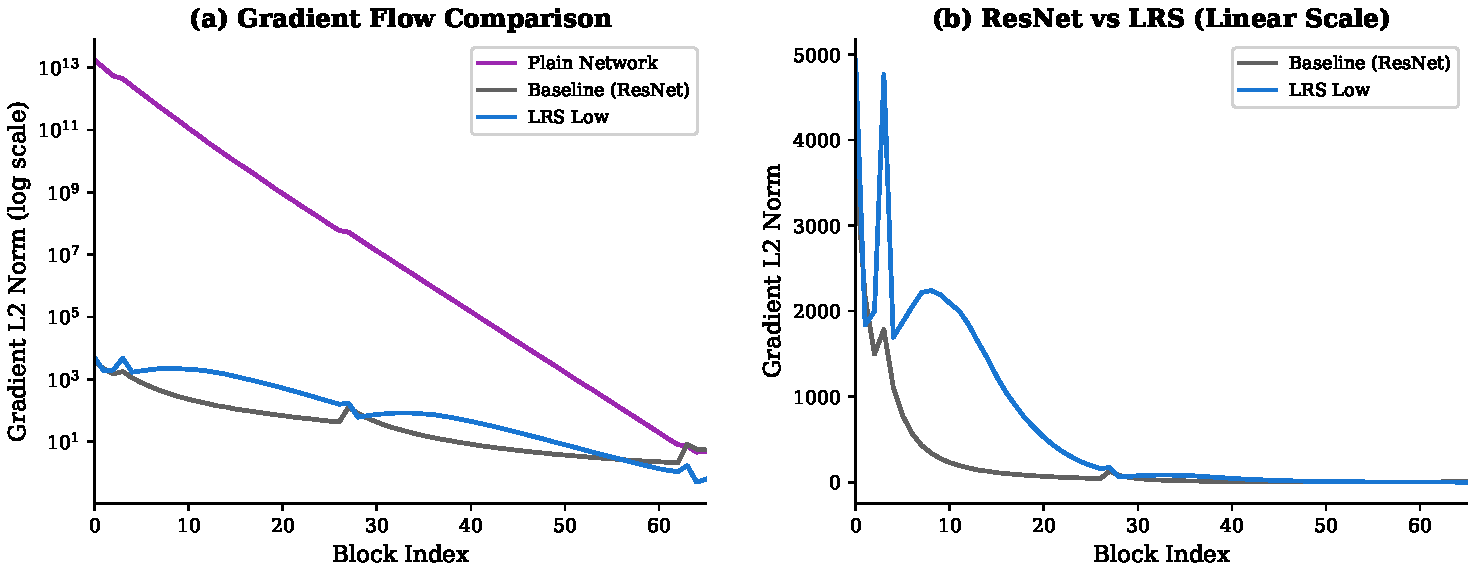
\includegraphics[width=\linewidth]{figures/fig0_gradient_flow.pdf}
    \caption{Per-block gradient L2 norms at initialization for ResNet-200 on CIFAR-100. (a) Plain networks without skip connections cannot self-select depth---gradients explode to $>10^{13}$ in early blocks. Skip connections stabilize the gradient distribution. (b--c) With LRS, late-block gradients decay toward zero, reflecting the network's learned choice $\alpha_i \approx 0$: those blocks are not used.}
    \label{fig:gradient_flow}
\end{figure}

\emph{(b) ResNets autonomously compress effective depth.} Across four depths ($50, 101, 152, 200$), two CIFAR datasets, and ImageNet at depths $50$ and $101$, three seeds each, the mean converged $\alpha$ decreases systematically with nominal depth ($0.34 \to 0.11$ on CIFAR-100 as depth grows $50 \to 200$). At the per-block level, a 200-layer network maintains $\alpha > 0.3$ in only 5--6 of 66 blocks. The threshold-free metric $D_\text{eff} = \sum_i \alpha_i$ confirms that quadrupling blocks ($16 \to 66$) increases effective depth by only $40\%$ ($5.4 \to 7.5$). The network is given depth and chooses to ignore most of it.

\emph{(c) The selected depth is intrinsic, not an artifact.} Three controls argue against optimization-induced bias. First, identity initialization of the residual branch yields nearly identical converged $\alpha$ ($0.114$ vs.\ $0.118$ for random init), showing the result does not depend on the starting point. Second, $\alpha$-guided block pruning validates the measurement: blocks with $\alpha < 0.03$ can be removed without retraining and incur \emph{zero} accuracy loss; pruning $56\%$ of blocks ($\alpha < 0.08$) followed by 10 epochs of fine-tuning recovers $76.22\%$ from the original $80.54\%$. Third, residual-favoring initialization ($\alpha_0 \approx 0.88$) causes catastrophic training failure at depth 200 (CIFAR-100: $37.50\pm29.20\%$), confirming that the identity-favored regime is not optional but necessary.

\textbf{Contributions.} (1) We propose that ResNets train successfully because of self-selection of effective depth, made possible by skip connections; LRS makes this measurable. (2) We empirically establish a depth--$\alpha$ scaling law that holds across CIFAR-10, CIFAR-100, and ImageNet at multiple depths. (3) We validate that the measurement is semantically meaningful through pruning, identity-init invariance, and initialization sensitivity analyses. (4) We reframe the degradation problem: it is not failure to be solved, but the network correctly refusing to use depth it does not need.

Code and all experimental results are available at \url{https://github.com/Wlsghdh/Learnable_Residual_Scaling}.

%% ============================================================
\section{Related Work}
\label{sec:related}

\subsection{Residual Networks and Skip Connections}

ResNet~\cite{he2016deep} introduced skip connections to alleviate gradient vanishing in deep networks. He et al.~\cite{he2016identity} further showed that identity mappings (pre-activation ResNet) improve gradient flow. Highway Networks~\cite{srivastava2015highway} proposed gated information flow prior to ResNet, but ResNet's simpler additive shortcut proved more effective in practice. Veit et al.~\cite{veit2016residual} reinterpreted ResNets as implicit ensembles of paths with varying lengths, showing that effective paths are much shorter than the nominal depth.

\subsection{Residual Scaling Methods}

Several works have explored adjusting the magnitude of the residual branch (Table~\ref{tab:comparison}).

\textbf{ReZero}~\cite{bachlechner2021rezero} initializes a scalar multiplier $\alpha = 0$ on the residual branch ($y = x + \alpha F(x)$), starting from identity to stabilize Transformer training.

\textbf{SkipInit}~\cite{de2020batch} similarly applies a learnable scalar to the residual branch, demonstrating that batch normalization biases residual blocks toward identity.

\textbf{Fixup}~\cite{zhang2019fixup} initializes the last layer of the residual branch to zero and proposes training without normalization through proper scaling.

\textbf{LayerScale}~\cite{touvron2021going} introduces per-channel learnable scaling vectors in Vision Transformers to stabilize training of deep ViTs.

All these methods adjust only $F(x)$ while keeping the identity connection $x$ fixed at weight 1. In contrast, LRS learns the \textbf{relative weight of both} $F(x)$ and $x$ through a single parameter, enabling direct measurement of each block's contribution.

\begin{table}[t]
\centering
\caption{Comparison of residual scaling methods. Only LRS measures the relative ratio between $F(x)$ and $x$, making it suitable as an analytical tool for effective depth.}
\label{tab:comparison}
\begin{tabular}{lccc}
\toprule
\textbf{Method} & \textbf{Formulation} & \textbf{Measurable} & \textbf{Key Difference} \\
\midrule
ReZero & $y = x + \alpha F(x)$ & $|F(x)|$ scale & $x$ weight fixed at 1 \\
SkipInit & $y = x + \alpha F(x)$ & $|F(x)|$ scale & $x$ weight fixed at 1 \\
LayerScale & $y = x + \Lambda F(x)$ & Per-ch. $|F(x)|$ & $x$ weight fixed at 1 \\
Fixup & $y = x + \alpha F(x)$ & $|F(x)|$ scale & Zero init last layer \\
\textbf{LRS (ours)} & $\mathbf{y = \alpha F(x) + (1{-}\alpha)x}$ & $\mathbf{F(x):x}$ \textbf{ratio} & \textbf{Both sides adjusted} \\
\bottomrule
\end{tabular}
\end{table}

\subsection{Comparison with Highway Networks}

A natural concern is whether LRS differs meaningfully from gated shortcuts proposed in Highway Networks~\cite{srivastava2015highway}, where $y = T(x)\cdot F(x) + (1 - T(x))\cdot x$ with $T(x) = \sigma(W_g x + b_g)$. The distinction is structural and central to our analysis. Highway's transform gate $T(x)$ is \emph{input-dependent}: every input produces a different gate value, so per-block usage cannot be summarized by a single number. LRS instead uses an \emph{input-independent scalar} $\alpha = \sigma(\theta)$, deliberately removing input dependency to obtain a per-block measurement. This is a methodological choice for interpretability, not a performance optimization: a single $\alpha$ per block makes ``how much does this block transform its input'' a well-defined quantity, enabling the depth--$\alpha$ scaling law, the per-block distribution analysis, and the pruning validation in Sections~\ref{sec:perblock}--\ref{sec:pruning}. Highway gates, by contrast, would require aggregating over input distributions to produce a comparable scalar---losing the very interpretability that motivates our design.

\subsection{Effective Depth and Network Redundancy}

The concept of effective depth has been explored from multiple angles. Huang et al.~\cite{huang2016deep} proposed stochastic depth, randomly dropping residual blocks during training, showing that not all blocks are needed. The lottery ticket hypothesis~\cite{frankle2019lottery} demonstrated that large networks contain small subnetworks that can match the full network's performance. The closest prior work is Veit et al.~\cite{veit2016residual}, which interpreted ResNets as ensembles of paths and showed empirically that effective paths are much shorter than the nominal depth.

However, prior evidence is \emph{indirect}: path-ensemble analysis relies on counting paths of various lengths, and lesion studies infer importance by deleting blocks and measuring degradation. The question ``how much does block $i$ actually contribute'' is answered only inferentially.  Our work provides a \emph{direct, per-block, quantitative measurement} of the same phenomenon: the learned $\alpha_i$ values are themselves the blocks' contributions, observable without any post-hoc analysis. This direct measurability enables three things prior work could not provide: (i) a quantitative scaling law $\bar{\alpha}(L)$ relating mean usage to depth, (ii) a threshold-free effective-depth metric $D_\text{eff} = \sum_i \alpha_i$, and (iii) a principled pruning criterion ($\alpha$-thresholding) that we validate by showing $\alpha < 0.03$ blocks can be removed with zero accuracy loss (Section~\ref{sec:pruning}). LRS thus complements Veit et al.\ by replacing inference with observation.

%% ============================================================
\section{Method}
\label{sec:method}

\subsection{Learnable Residual Scaling}

We redefine the standard residual block output $y = F(x) + x$ as:
\begin{equation}
    y = \alpha \cdot F(x) + (1 - \alpha) \cdot x
    \label{eq:lrs}
\end{equation}
where $\alpha = \sigma(\theta)$, $\theta$ is a learnable scalar parameter per block, and $\sigma$ is the sigmoid function constraining $\alpha \in (0, 1)$.

\textbf{Design rationale.} The sigmoid parameterization serves two purposes. First, since $\alpha + (1 - \alpha) = 1$, the \textbf{relative ratio} between $F(x)$ and $x$ is directly interpretable: $\alpha = 0.14$ means the block allocates 14\% weight to the transformation and 86\% to the identity. Second, the bounded range ensures numerical stability.

The semantics of $\alpha$ provide a natural definition of effective depth:
\begin{itemize}
    \item $\alpha \to 0$: The block is effectively bypassed ($y \approx x$); it does not contribute to the network's effective depth.
    \item $\alpha = 0.5$: Equal ratio, equivalent to the standard ResNet block.
    \item $\alpha \to 1$: The block performs a full transformation ($y \approx F(x)$).
\end{itemize}

A block with small $\alpha$ is one that the network has chosen to largely skip. The \textbf{effective depth} of the network is the number of blocks with $\alpha$ above a meaningful threshold.

\begin{figure}[t]
    \centering
    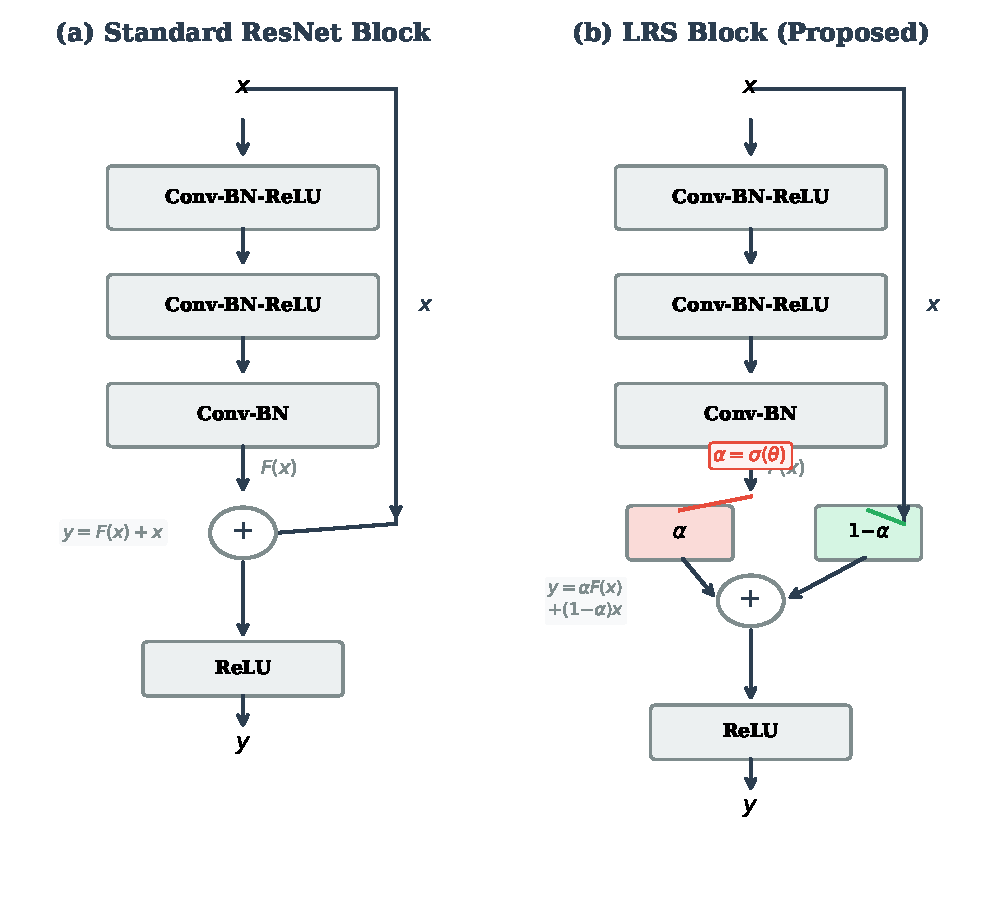
\includegraphics[width=0.85\linewidth]{figures/fig1_block_diagram.pdf}
    \caption{Computation graph of an LRS block. The learnable parameter $\alpha = \sigma(\theta) \in (0,1)$ controls the relative contribution of the residual transformation $F(x)$ and the identity shortcut $x$. After training, $\alpha$ reveals whether the block actively transforms its input or effectively acts as an identity bypass.}
    \label{fig:lrs_block}
\end{figure}

\subsection{Gradient Flow Analysis}

The backward pass through an LRS block yields:
\begin{equation}
    \frac{\partial \mathcal{L}}{\partial x} = \frac{\partial \mathcal{L}}{\partial y} \left[ (1 - \alpha) + \alpha \cdot F'(x) \right]
    \label{eq:grad}
\end{equation}

The total gradient through $L$ blocks:
\begin{equation}
    \frac{\partial \mathcal{L}}{\partial x_0} = \frac{\partial \mathcal{L}}{\partial y_L} \cdot \prod_{i=1}^{L} \left[ (1 - \alpha_i) + \alpha_i \cdot F'_i(x_i) \right]
    \label{eq:total_grad}
\end{equation}

This product structure explains the depth--$\alpha$ relationship. For the product to remain stable across $L$ blocks, each factor $(1 - \alpha_i) + \alpha_i F'_i$ must be close to 1. When $\alpha_i$ is small, the factor approaches $(1 - \alpha_i) \approx 1$ regardless of $F'_i$, ensuring gradient stability. As $L$ grows, smaller $\alpha_i$ values are needed to maintain the product near unity. This provides the theoretical basis for why deeper networks should converge to smaller $\alpha$ values.

Conversely, when $\alpha_i$ is large (close to 1), the factor becomes $\approx F'_i$, and the gradient product degenerates to that of a plain (non-residual) network, which is prone to vanishing gradients. This explains why residual-favoring initialization ($\alpha_0 \approx 0.88$) leads to training collapse at extreme depth.

\subsection{Initialization Variants}

We experiment with three initialization strategies (Table~\ref{tab:init_variants}) to study convergence and sensitivity:

\begin{table}[t]
\centering
\caption{LRS model variants by $\alpha$ initialization. All three start from different points to test whether $\alpha$ converges to the same optimum.}
\label{tab:init_variants}
\begin{tabular}{lccc}
\toprule
\textbf{Variant} & $\theta_0$ & $\alpha_0$ & \textbf{Initial Bias} \\
\midrule
LRS Low  & $-2.0$ & $\approx 0.12$ & Identity-favoring \\
LRS Mid  & $0.0$  & $0.50$         & Balanced (standard ResNet) \\
LRS High & $+2.0$  & $\approx 0.88$ & Residual-favoring \\
\bottomrule
\end{tabular}
\end{table}

These three initializations serve as probes: if the optimization landscape has a single basin, all three should converge to the same $\alpha$; if initialization matters, we expect divergence, revealing the role of initial conditions in determining effective depth.

%% ============================================================
\section{Experiments}
\label{sec:experiments}

\subsection{Experimental Setup}
\label{sec:setup}

\textbf{Datasets.} CIFAR-10 (10 classes, 50K/10K train/test) and CIFAR-100 (100 classes, 50K/10K) for systematic analysis; ImageNet (1000 classes, 1.28M/50K) for large-scale validation.

\textbf{Architectures.} Bottleneck ResNet-50/101/152/200 for CIFAR experiments; ResNet-50 for ImageNet. The number of residual blocks per depth is: 50$\to$16, 101$\to$33, 152$\to$50, 200$\to$66.

\textbf{Training (CIFAR).} SGD with momentum 0.9 and weight decay $10^{-4}$; initial learning rate 0.1 with cosine annealing; 5-epoch linear warmup; 100 total epochs; batch size 128.

\textbf{Training (ImageNet).} SGD with momentum 0.9 and weight decay $10^{-4}$; initial learning rate 0.1 with cosine annealing; 5-epoch warmup; 100 epochs; batch size 256.

\textbf{Seeds and reporting.} All CIFAR experiments use 3 random seeds (42, 123, 456). We report mean $\pm$ standard deviation. ImageNet experiments use a single seed due to computational cost.

\textbf{Models.} Five primary models are evaluated: Baseline (standard ResNet), LRS Low ($\alpha_0 \approx 0.12$), LRS Mid ($\alpha_0 = 0.50$), LRS High ($\alpha_0 \approx 0.88$), and ReZero ($\alpha_0 = 0$, $y = x + \alpha F(x)$). For comparison with existing methods, we additionally evaluate SkipInit, Fixup, and LayerScale.

\subsection{Alpha Convergence Across Depths}
\label{sec:alpha_convergence}

We first examine the central question: how does the network's preferred $\alpha$ change with depth? Table~\ref{tab:depth_alpha} presents the mean converged $\alpha$ values on CIFAR-100 for all three LRS initialization variants, averaged over 3 seeds.

\begin{table}[t]
\centering
\caption{Mean converged $\alpha$ values by depth on CIFAR-100 (3-seed average). Despite starting from very different initial values ($\alpha_0 = 0.12, 0.50, 0.88$), the Low and Mid variants converge to similar final values at each depth, while High diverges at greater depths.}
\label{tab:depth_alpha}
\begin{tabular}{lcccc}
\toprule
\textbf{Depth} & \textbf{Blocks} & \textbf{LRS Low} & \textbf{LRS Mid} & \textbf{LRS High} \\
\midrule
50  & 16 & 0.34 & 0.35 & 0.36 \\
101 & 33 & 0.18 & 0.20 & 0.21 \\
152 & 50 & 0.13 & 0.15 & 0.23 \\
200 & 66 & 0.11 & 0.13 & 0.28 \\
\bottomrule
\end{tabular}
\end{table}

Several important observations emerge:

\textbf{Systematic decrease with depth.} The converged $\alpha$ decreases monotonically with depth across all initialization variants. For LRS Low, $\alpha$ drops from 0.34 (depth 50) to 0.11 (depth 200), indicating that the network allocates only 11\% weight to block transformations in the deepest configuration. This means each block's contribution shrinks as more blocks are added.

\textbf{Partial convergence across initializations.} At depth 50, all three variants converge to nearly identical values (0.34--0.36), indicating a well-defined optimum. However, at depth 200, the convergence breaks down: LRS High settles at 0.28, significantly above the 0.11--0.13 range of Low and Mid. This divergence is coupled with severe performance degradation (Section~\ref{sec:init_sensitivity}), indicating that LRS High becomes trapped in a suboptimal basin at extreme depth.

\textbf{Data independence.} The converged $\alpha$ values are highly similar between CIFAR-10 and CIFAR-100 (not shown separately for brevity), suggesting that the depth--$\alpha$ relationship is governed by architectural properties rather than task complexity.

\begin{figure}[t]
    \centering
    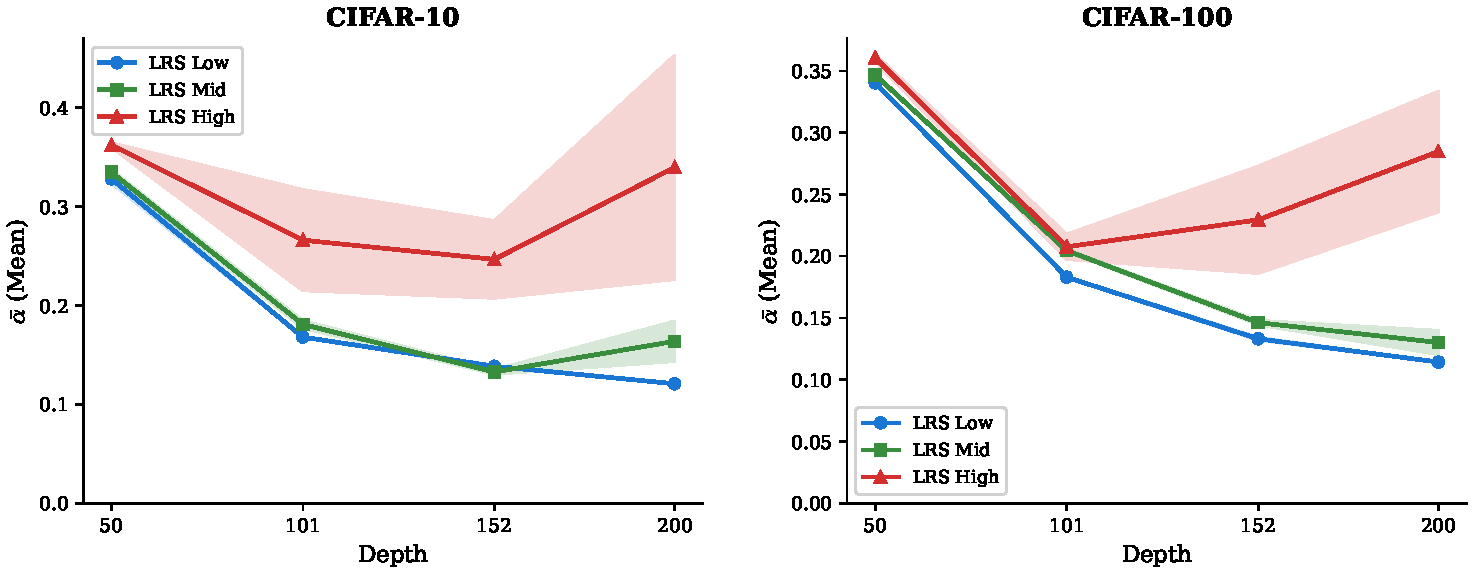
\includegraphics[width=0.85\linewidth]{figures/fig2_alpha_depth.pdf}
    \caption{Mean converged $\alpha$ as a function of network depth for three initialization variants on CIFAR-100. At shallow depths, all initializations converge to similar values; at extreme depths, High initialization diverges due to optimization difficulties.}
    \label{fig:alpha_convergence}
\end{figure}

\subsection{Alpha Trajectory During Training}
\label{sec:alpha_trajectory}

Figure~\ref{fig:alpha_trajectory} shows how the mean $\alpha$ evolves during the course of training. All three initializations show rapid early adjustment: LRS Low increases slightly from 0.12, LRS Mid decreases from 0.50, and LRS High decreases from 0.88 (when training succeeds). The trajectories largely stabilize within the first 20--30 epochs, with fine-tuning continuing until the end of training.

At depth 200, the LRS High trajectory reveals the failure mode: $\alpha$ decreases slowly but fails to reach the values achieved by Low and Mid, remaining stuck at approximately 0.28. The network cannot recover from the initial gradient degradation caused by the high $\alpha$ values.

\begin{figure}[t]
    \centering
    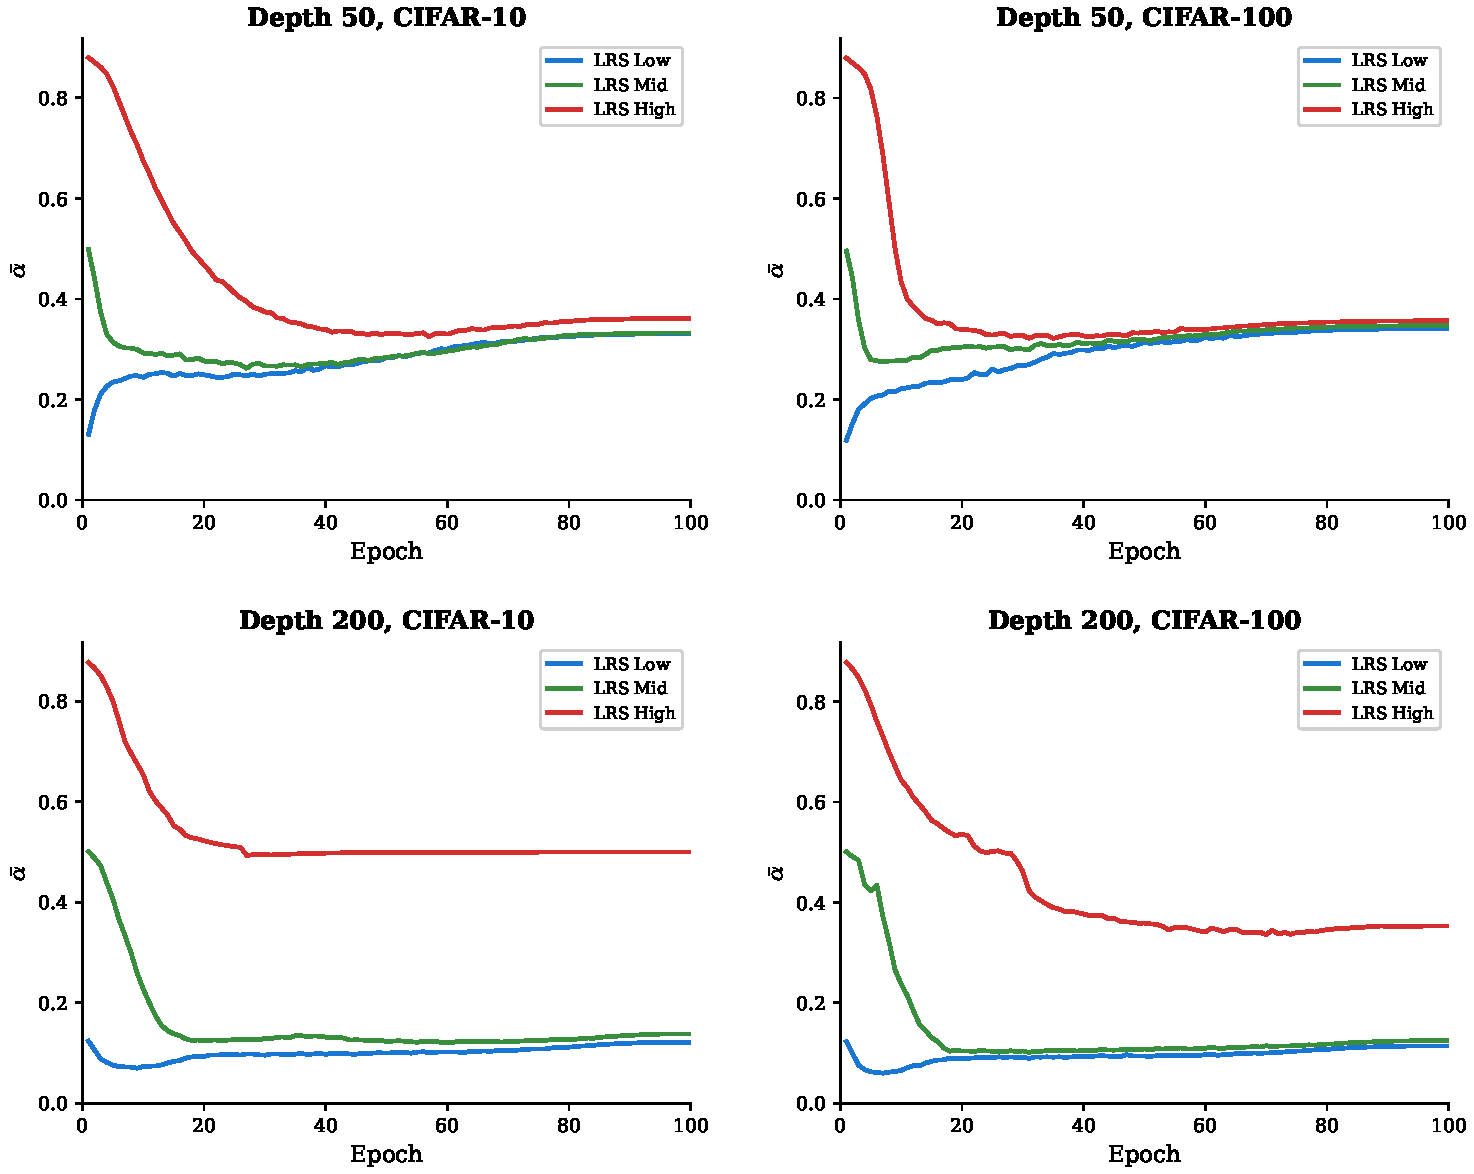
\includegraphics[width=\linewidth]{figures/fig3_alpha_trajectory.pdf}
    \caption{Mean $\alpha$ trajectories during training across epochs. Left: successful convergence from different starting points at moderate depth. Right: at depth 200, LRS High fails to converge to the optimal range, remaining trapped at a suboptimal $\alpha \approx 0.28$.}
    \label{fig:alpha_trajectory}
\end{figure}

\subsection{Per-Block Alpha Distribution}
\label{sec:perblock}

The mean $\alpha$ value across all blocks hides important structure. Figure~\ref{fig:perblock_alpha} shows the per-block $\alpha$ distribution for a 200-layer network (66 blocks, LRS Low, CIFAR-100).

The distribution reveals a striking pattern:

\textbf{Downsampling blocks have high $\alpha$.} The first block of each stage (where spatial downsampling occurs and channel dimensions change) maintains $\alpha$ values between 0.42 and 0.96, approximately 5$\times$ the average. These blocks perform essential feature transformations that cannot be bypassed.

\textbf{Normal blocks have low $\alpha$.} Within each stage, non-downsampling blocks have $\alpha$ values of 0.06--0.15, and these values tend to decrease toward the end of the stage. Most of these blocks are near-identity operations.

\textbf{Decreasing $\alpha$ within stages.} Within a given stage, blocks further from the downsampling point tend to have progressively smaller $\alpha$ values, suggesting diminishing marginal contribution.

\begin{figure}[t]
    \centering
    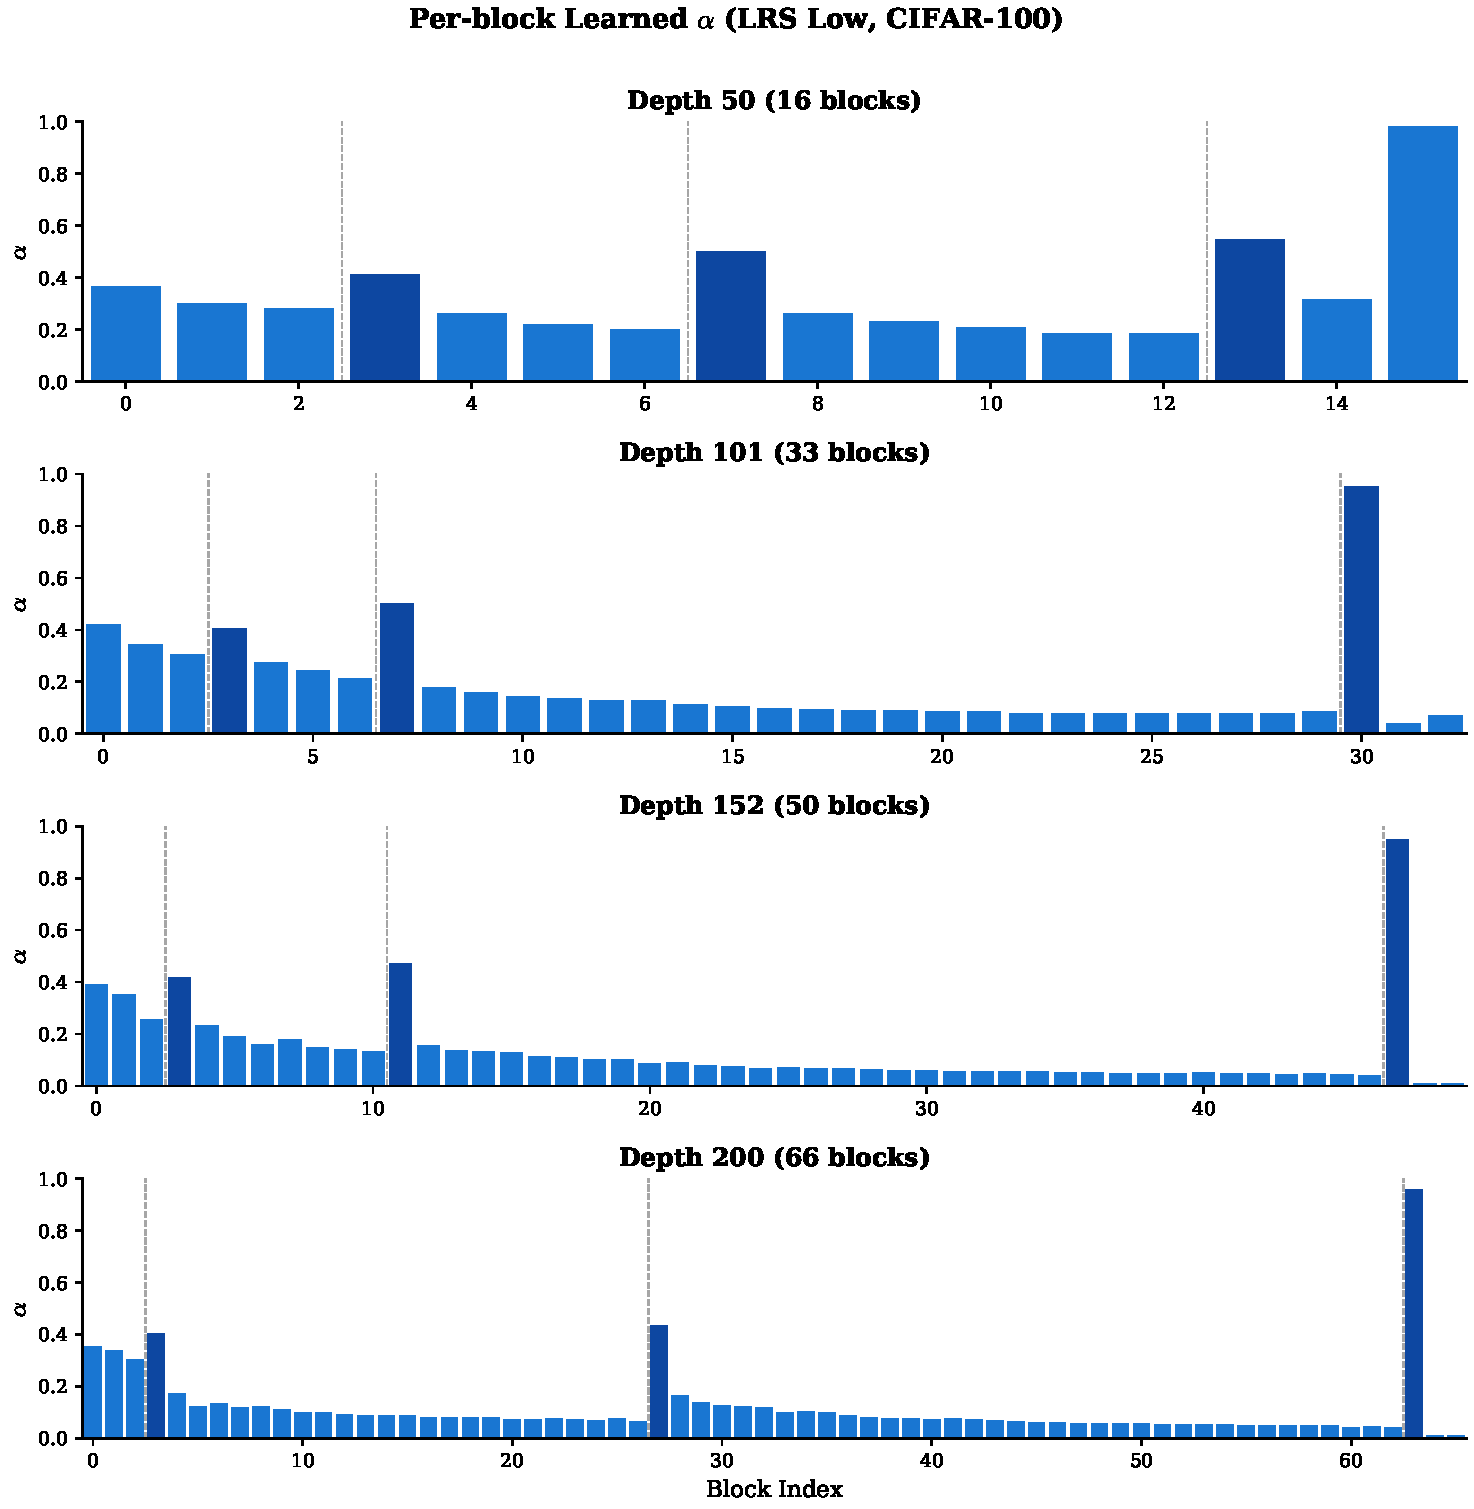
\includegraphics[width=\linewidth]{figures/fig4_perblock_alpha.pdf}
    \caption{Per-block $\alpha$ values for a 200-layer ResNet (66 blocks, LRS Low, CIFAR-100). Stage boundaries (downsampling blocks) are marked with dashed lines. Downsampling blocks maintain high $\alpha$ while most within-stage blocks converge to near-zero values.}
    \label{fig:perblock_alpha}
\end{figure}

\begin{figure}[t]
    \centering
    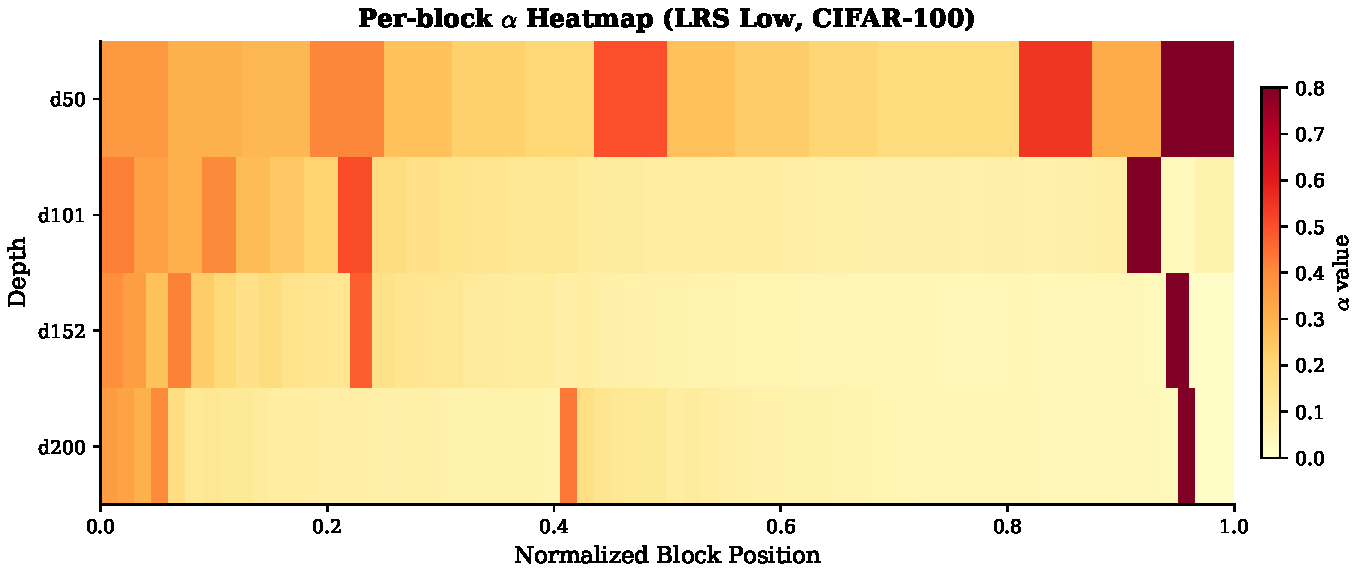
\includegraphics[width=0.85\linewidth]{figures/fig8_heatmap.pdf}
    \caption{Detailed view of per-block $\alpha$ distributions grouped by stage. The consistent pattern of high $\alpha$ at stage boundaries followed by decay within each stage is evident across all four stages.}
    \label{fig:perblock_detail}
\end{figure}

\subsection{Effective Depth Analysis}
\label{sec:effective_depth}

The per-block $\alpha$ distribution enables a direct measurement of \emph{effective depth}---the number of blocks that meaningfully transform their input. Using $\alpha > 0.3$ as a threshold (blocks contributing more than 30\% transformation), we find:

\begin{table}[t]
\centering
\caption{Effective depth analysis for ResNet-200 (66 blocks) on CIFAR-100, LRS Low. The network uses only a small fraction of its nominal depth.}
\label{tab:effective_depth}
\begin{tabular}{lcc}
\toprule
\textbf{Metric} & \textbf{Value} & \textbf{Interpretation} \\
\midrule
Nominal blocks & 66 & Total residual blocks \\
Blocks with $\alpha > 0.3$ & 5--6 & Actively transforming \\
Effective depth ratio & $\sim$8\% & Fraction of blocks used \\
Mean $\alpha$ (normal blocks) & 0.06--0.15 & Near-identity \\
Mean $\alpha$ (downsampling blocks) & 0.42--0.96 & Active transformation \\
\bottomrule
\end{tabular}
\end{table}

This finding has a remarkable implication: \textbf{a 200-layer ResNet autonomously selects an effective depth of approximately 5--6 blocks}. The remaining 60+ blocks serve primarily as identity shortcuts, passing information through with minimal transformation. The network has, in effect, chosen to be shallow despite being given the capacity to be deep.

This is consistent with the ensemble interpretation of Veit et al.~\cite{veit2016residual}, who showed that effective paths in ResNets are much shorter than the full network depth. LRS provides a direct, per-block measurement of this phenomenon.

\textbf{Threshold sensitivity.} The choice of $\alpha > 0.3$ as the threshold for ``active'' blocks is admittedly arbitrary. To address this concern, we present two complementary analyses.

First, Table~\ref{tab:threshold_sensitivity} shows effective depth across a range of thresholds. Regardless of the threshold chosen, two patterns remain invariant: (1) effective depth ratio decreases monotonically with nominal depth, and (2) the gap between shallow and deep networks is substantial at every threshold.

\begin{table}[t]
\centering
\caption{Effective depth ratio (\% of blocks with $\alpha$ above threshold) for LRS Low on CIFAR-100 (3-seed average). The pattern of decreasing effective depth with increasing nominal depth is consistent across all thresholds.}
\label{tab:threshold_sensitivity}
\begin{tabular}{lcccc}
\toprule
\textbf{Threshold} & \textbf{Depth 50} & \textbf{Depth 101} & \textbf{Depth 152} & \textbf{Depth 200} \\
\midrule
$\alpha > 0.10$ & 100\% & 54\% & 40\% & 28\% \\
$\alpha > 0.20$ & 83\% & 27\% & 15\% & 10\% \\
$\alpha > 0.30$ & 40\% & 18\% & 11\% & 7\% \\
$\alpha > 0.40$ & 25\% & 12\% & 7\% & 5\% \\
\bottomrule
\end{tabular}
\end{table}

Second, we define a threshold-free metric: $D_\text{eff} = \sum_{i=1}^{N} \alpha_i$, which represents the effective depth as the sum of all block contributions. This metric requires no arbitrary cutoff:

\begin{table}[t]
\centering
\caption{Threshold-free effective depth ($D_\text{eff} = \sum \alpha_i$) for LRS Low on CIFAR-100. Although the number of blocks increases 4$\times$ from depth 50 to 200, $D_\text{eff}$ increases only 1.4$\times$.}
\label{tab:deff}
\begin{tabular}{lccc}
\toprule
\textbf{Depth} & \textbf{Blocks ($N$)} & $\mathbf{D_\text{eff} = \sum \alpha_i}$ & $\mathbf{D_\text{eff}/N}$ \\
\midrule
50  & 16 & 5.4 & 34.0\% \\
101 & 33 & 6.0 & 18.3\% \\
152 & 50 & 6.7 & 13.3\% \\
200 & 66 & 7.5 & 11.4\% \\
\bottomrule
\end{tabular}
\end{table}

The $D_\text{eff}$ metric confirms the main finding without any threshold: quadrupling the number of blocks (16 $\to$ 66) increases the effective depth by only 40\% (5.4 $\to$ 7.5). The network adds blocks but barely uses them.

\begin{figure}[t]
    \centering
    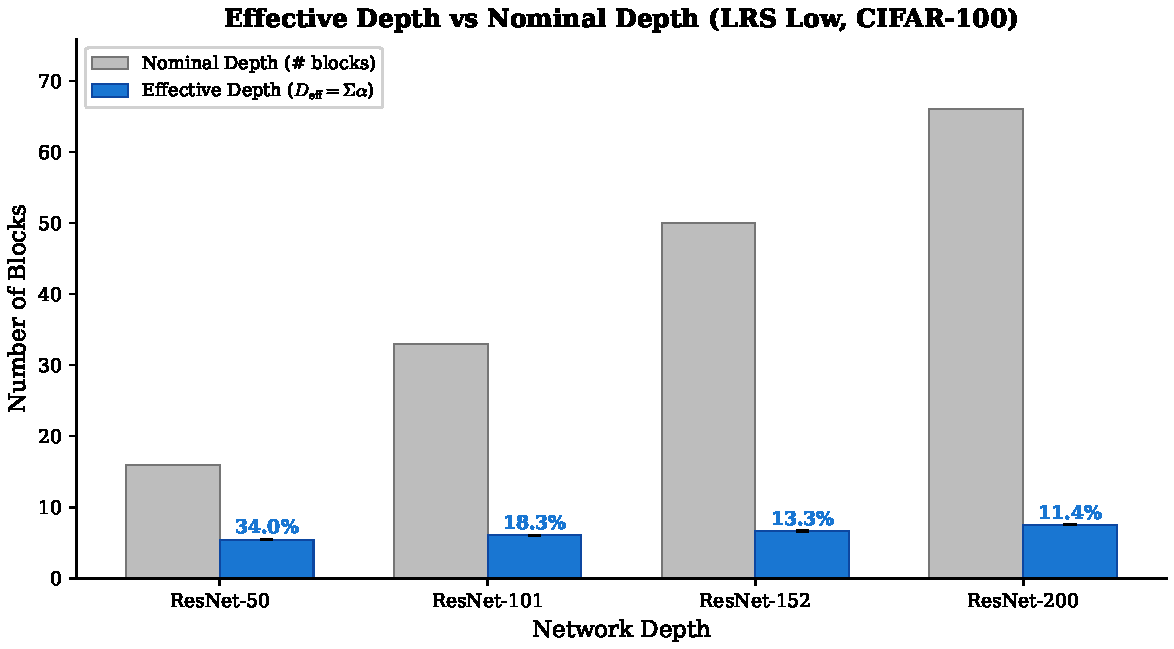
\includegraphics[width=0.85\linewidth]{figures/fig5_effective_depth.pdf}
    \caption{Effective depth visualization. Each block is colored by its $\alpha$ value: dark blocks ($\alpha > 0.3$) actively transform the input; light blocks ($\alpha < 0.15$) are near-identity bypasses. Only 5--6 out of 66 blocks in ResNet-200 are ``dark,'' revealing that the network's effective depth is roughly 8\% of its nominal depth.}
    \label{fig:effective_depth}
\end{figure}

\subsection{Initialization Sensitivity and LRS High Failure}
\label{sec:init_sensitivity}

The three LRS initializations reveal dramatic differences in training stability as depth increases. Tables~\ref{tab:cifar10} and~\ref{tab:cifar100} present the full accuracy results.

\begin{table}[t]
\centering
\caption{Test accuracy (\%) on CIFAR-10 (3-seed mean $\pm$ std). LRS High shows progressive degradation and catastrophic failure at depth 200.}
\label{tab:cifar10}
\begin{tabular}{lccccc}
\toprule
\textbf{Depth} & \textbf{Baseline} & \textbf{LRS Low} & \textbf{LRS Mid} & \textbf{LRS High} & \textbf{ReZero} \\
\midrule
50  & 94.53$\pm$0.14 & \textbf{94.83$\pm$0.13} & 94.77$\pm$0.03 & 94.27$\pm$0.17 & 94.60$\pm$0.28 \\
101 & 95.37$\pm$0.11 & \textbf{95.44$\pm$0.12} & 95.15$\pm$0.11 & 94.28$\pm$0.29 & 95.38$\pm$0.21 \\
152 & 95.95$\pm$0.06 & 95.73$\pm$0.10 & 95.60$\pm$0.15 & 93.78$\pm$0.87 & \textbf{95.99$\pm$0.06} \\
200 & 95.98$\pm$0.15 & \textbf{96.10$\pm$0.12} & 94.36$\pm$0.92 & 67.25$\pm$43.65 & 96.02$\pm$0.16 \\
\bottomrule
\end{tabular}
\end{table}

\begin{table}[t]
\centering
\caption{Test accuracy (\%) on CIFAR-100 (3-seed mean $\pm$ std). The progressive failure of LRS High is even more pronounced on this harder task.}
\label{tab:cifar100}
\begin{tabular}{lccccc}
\toprule
\textbf{Depth} & \textbf{Baseline} & \textbf{LRS Low} & \textbf{LRS Mid} & \textbf{LRS High} & \textbf{ReZero} \\
\midrule
50  & 77.18$\pm$0.36 & 77.02$\pm$0.20 & 76.72$\pm$0.40 & 75.22$\pm$0.45 & 76.12$\pm$0.09 \\
101 & \textbf{79.29$\pm$0.23} & 78.85$\pm$0.14 & 78.34$\pm$0.19 & 75.16$\pm$1.69 & 78.04$\pm$0.48 \\
152 & \textbf{80.42$\pm$0.22} & 80.28$\pm$0.38 & 78.57$\pm$0.60 & 71.66$\pm$3.40 & 79.72$\pm$0.10 \\
200 & \textbf{80.72$\pm$0.17} & 80.65$\pm$0.01 & 76.07$\pm$1.59 & 37.50$\pm$29.20 & 80.14$\pm$0.17 \\
\bottomrule
\end{tabular}
\end{table}

The results reveal a clear hierarchy of initialization safety:

\textbf{LRS Low ($\alpha_0 \approx 0.12$)} performs on par with or slightly above the baseline at all depths, with low variance across seeds. It achieves the best result at depth 200 on CIFAR-10 (96.10\%) and near-best on CIFAR-100 (80.65\%).

\textbf{LRS Mid ($\alpha_0 = 0.50$)} is stable at moderate depths but degrades at depth 200 (CIFAR-100: 76.07$\pm$1.59\%), with increasing variance signaling optimization instability.

\textbf{LRS High ($\alpha_0 \approx 0.88$)} shows progressive degradation with depth, culminating in catastrophic failure at depth 200: 67.25$\pm$43.65\% on CIFAR-10 and 37.50$\pm$29.20\% on CIFAR-100. The enormous standard deviation indicates that some seeds fail completely while others partially recover.

The mechanism of failure is clear from the gradient analysis (Equation~\ref{eq:total_grad}): with $\alpha_0 = 0.88$, the identity component of each gradient factor is only $1 - 0.88 = 0.12$. Through 66 blocks, the gradient preservation baseline is $0.12^{66}$, which is astronomically small, making learning impossible without rapid $\alpha$ adjustment. But rapid $\alpha$ adjustment itself requires gradients---creating a chicken-and-egg problem that leads to training collapse.

\begin{figure}[t]
    \centering
    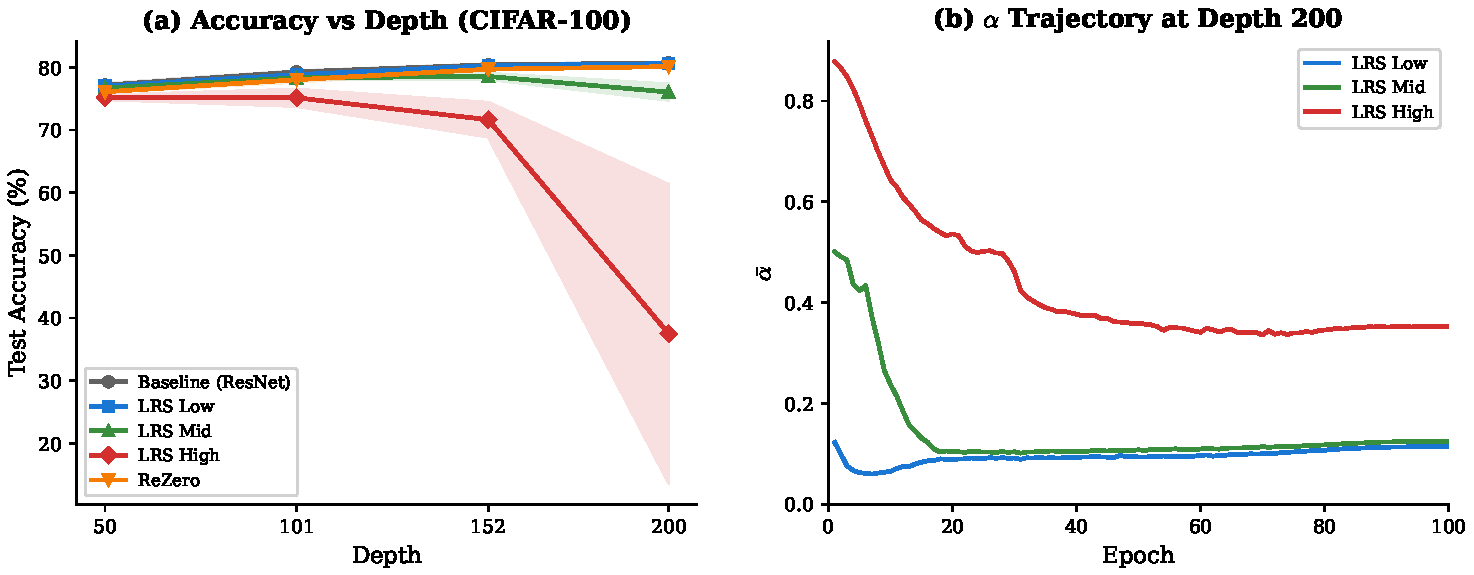
\includegraphics[width=0.85\linewidth]{figures/fig6_init_failure.pdf}
    \caption{Accuracy across depths for three LRS initializations on CIFAR-100. LRS Low remains stable and competitive with the baseline at all depths. LRS High degrades progressively and collapses at depth 200.}
    \label{fig:init_sensitivity}
\end{figure}

\subsection{Fixed vs.\ Learned Alpha}
\label{sec:fixed_alpha}

To validate that \emph{learning} $\alpha$ is essential---not just using a small fixed value---we compare learned LRS with fixed-$\alpha$ variants at depth 152 on CIFAR-100.

\begin{table}[t]
\centering
\caption{Fixed $\alpha$ vs.\ learned $\alpha$ at depth 152 on CIFAR-100. A fixed value, even if close to the learned mean, cannot match the performance of per-block learning.}
\label{tab:fixed_alpha}
\begin{tabular}{lcc}
\toprule
\textbf{Configuration} & \textbf{Accuracy (\%)} & \textbf{Notes} \\
\midrule
Learned (LRS Low) & \textbf{80.28} & Per-block $\alpha$, mean $\approx 0.13$ \\
Fixed $\alpha = 0.1$ & 79.81 & Close to learned mean \\
Fixed $\alpha = 0.3$ & 67.94 & Moderate transformation \\
Fixed $\alpha = 0.5$ & 44.19 & Standard ResNet ratio \\
Fixed $\alpha = 0.7$ & 20.62 & Residual-favoring \\
\midrule
Baseline ($\alpha = 0.5$ implicit) & 80.42 & Standard ResNet (no LRS) \\
\bottomrule
\end{tabular}
\end{table}

The results are striking. First, $\alpha = 0.5$ (the standard ResNet ratio, applied uniformly with the complementary identity scaling) yields only 44.19\%, far worse than the baseline's 80.42\%. This is because the fixed-$\alpha$ formulation $y = 0.5 F(x) + 0.5 x$ explicitly halves both branches, unlike the standard ResNet's $y = F(x) + x$ which preserves full scale. This confirms that the LRS formulation is meaningful only when $\alpha$ is learned or set to a small value.

Second, even fixed $\alpha = 0.1$, which is close to the learned mean of 0.13, underperforms the learned variant by 0.47\%. This gap arises because learned LRS assigns high $\alpha$ to downsampling blocks (0.42--0.96) while keeping normal blocks near zero. A uniform fixed value cannot capture this heterogeneous structure.

\begin{figure}[t]
    \centering
    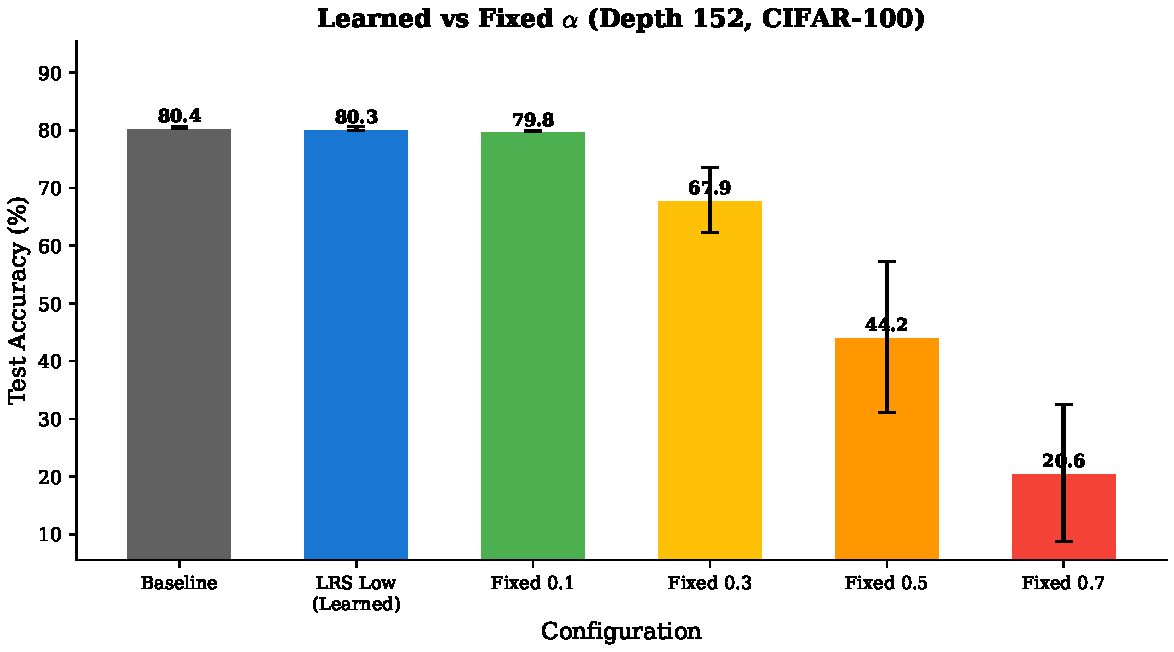
\includegraphics[width=0.85\linewidth]{figures/fig7_fixed_alpha.pdf}
    \caption{Accuracy as a function of fixed $\alpha$ at depth 152, CIFAR-100. The learned per-block $\alpha$ (dashed line) outperforms all fixed values, demonstrating that the heterogeneous block-wise structure is essential.}
    \label{fig:fixed_vs_learned}
\end{figure}

\subsection{Identity Initialization Analysis}
\label{sec:identity_init}

A natural hypothesis is that the low effective depth observed with LRS might be an artifact of the standard He initialization, which initializes the residual branch with random weights rather than an identity-preserving mapping. If the residual branch started as an identity transformation (providing a ``better starting point''), would the network choose to use more blocks?

To test this, we compare standard He initialization with partial and full identity initialization schemes. HybridA initializes layers 3 and 4 (the deeper stages) with identity-preserving weights while keeping He initialization for layers 1 and 2. We also test full identity initialization across all layers. Table~\ref{tab:identity_init} presents the results on CIFAR-100.

\begin{table}[t]
\centering
\caption{Effect of identity initialization on accuracy and learned $\alpha$ (CIFAR-100, 3-seed mean $\pm$ std). Full identity initialization catastrophically fails, while partial identity (HybridA) + LRS achieves the best accuracy---yet the effective depth remains unchanged.}
\label{tab:identity_init}
\begin{tabular}{lcccc}
\toprule
\textbf{Model} & \textbf{d152 Acc (\%)} & \textbf{d200 Acc (\%)} & \textbf{$\alpha$ mean (d200)} & \textbf{Active blocks} \\
\midrule
Baseline (He init) & 80.42$\pm$0.18 & 80.72$\pm$0.13 & --- & --- \\
LRS Low + He init & 80.28$\pm$0.31 & 80.65$\pm$0.01 & 0.114 & 5 / 66 \\
HybridA (Identity L3,4) & 80.02$\pm$0.26 & 80.40$\pm$0.17 & --- & --- \\
LRS Low + HybridA & \textbf{80.72$\pm$0.29} & \textbf{81.14$\pm$0.18} & 0.118 & 6 / 66 \\
ResNet (Full Identity) & 13.41$\pm$0.41 & 12.98$\pm$0.16 & --- & --- \\
\bottomrule
\end{tabular}
\end{table}

Several findings emerge from this experiment:

\textbf{Full identity initialization catastrophically fails.} When all residual branches are initialized as identity transformations, the network collapses to near-random performance (12.98\% at depth 200). Without the diversity provided by random initialization, the network cannot break symmetry and learn meaningful features.

\textbf{Partial identity initialization improves accuracy.} The combination of HybridA (identity initialization for the deeper stages 3 and 4) with LRS achieves the best accuracy across all configurations: 81.14\% at depth 200, surpassing both the standard baseline (80.72\%) and standard LRS Low (80.65\%).

\textbf{Effective depth is invariant to initialization.} Despite the improved accuracy, the learned $\alpha$ values are nearly identical between standard and identity initialization: 0.114 vs.\ 0.118 mean $\alpha$, with 5 vs.\ 6 active blocks (out of 66). The network converges to the same effective depth regardless of how the residual branch is initialized.

This result is significant because it rules out the hypothesis that low effective depth is an artifact of poor initialization. Even when the residual branch is initialized to perform identity transformations---providing a better starting point for learning useful transformations---the network converges to the same effective depth. This suggests that the low effective depth reflects the network's \emph{genuine preference}, not a limitation imposed by initialization.

\subsection{Block Pruning Validation}
\label{sec:pruning}

To directly validate that low-$\alpha$ blocks are genuinely redundant, we perform two pruning experiments. First, blocks with $\alpha$ below a threshold are replaced with identity mappings and accuracy is measured without retraining. Second, we apply 10 epochs of fine-tuning after pruning to allow the remaining blocks to adapt. Each bottleneck block comprises 6 layers (three convolutions and three batch normalizations).

\begin{table}[t]
\centering
\caption{Block pruning results on CIFAR-100 (ResNet-200, 66 blocks). ``No FT'' removes blocks and evaluates immediately; ``With FT'' applies 10 epochs of fine-tuning after removal.}
\label{tab:pruning}
\begin{tabular}{lcccccc}
\toprule
\textbf{Threshold} & \textbf{Removed} & \textbf{Layers} & \textbf{Kept} & \textbf{No FT} & \textbf{With FT} & $\mathbf{\Delta}$ \\
\midrule
None (original) & 0 & 0 & 66 & 80.54\% & --- & --- \\
$\alpha < 0.03$ & 2 (3\%) & 12 & 64 & 80.54\% & --- & \textbf{0.00} \\
$\alpha < 0.05$ & 10 (15\%) & 60 & 56 & 73.88\% & 79.53\% & \textbf{$-$1.01} \\
$\alpha < 0.08$ & 37 (56\%) & 222 & 29 & 3.97\% & 76.22\% & $-$4.32 \\
$\alpha < 0.10$ & 48 (73\%) & 288 & 18 & 3.13\% & 74.83\% & $-$5.71 \\
$\alpha < 0.15$ & 58 (88\%) & 348 & 8 & 3.63\% & 72.64\% & $-$7.90 \\
\bottomrule
\end{tabular}
\end{table}

The results reveal two important findings. First, blocks with $\alpha < 0.03$ are genuinely inactive: removing 2 blocks (12 layers) causes \textbf{zero accuracy loss}, confirming that $\alpha$ accurately identifies redundant blocks.

Second, fine-tuning dramatically improves recovery. Without fine-tuning, removing 15\% of blocks ($\alpha < 0.05$) drops accuracy by 6.66\%; with just 10 epochs of fine-tuning, the loss reduces to only \textbf{1.01\%}. Even removing 56\% of blocks recovers to 76.22\% (from 80.54\%), and removing 73\% still yields 74.83\%. This demonstrates that the network's computation is highly distributed: while individual low-$\alpha$ blocks contribute little, fine-tuning allows the remaining blocks to compensate, confirming the ensemble interpretation of Veit et al.~\cite{veit2016residual}.

\begin{figure}[t]
    \centering
    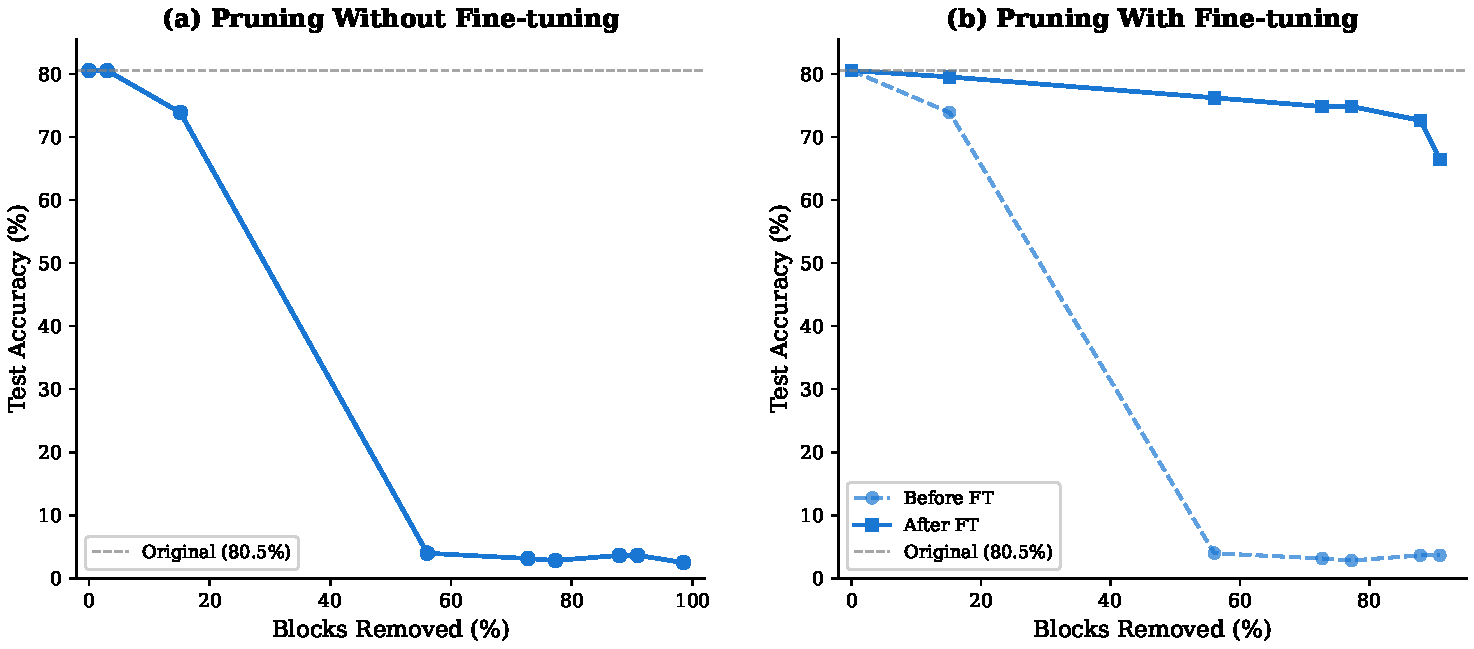
\includegraphics[width=\linewidth]{figures/fig11_pruning.pdf}
    \caption{Block pruning results for ResNet-200 on CIFAR-100. Left: without fine-tuning, only $\alpha < 0.03$ blocks can be removed safely. Right: with 10 epochs of fine-tuning, up to 15\% of blocks can be removed with less than 1\% accuracy loss, and even 56\% removal recovers to 76\%.}
    \label{fig:pruning}
\end{figure}

\subsection{Comparison with Existing Methods}
\label{sec:comparison_methods}

We compare LRS with established residual scaling methods at depth 152 on CIFAR-100, using 3 seeds for all methods (Table~\ref{tab:method_comparison}).

\begin{table}[t]
\centering
\caption{Comparison with existing residual scaling methods (depth 152, CIFAR-100, 3-seed mean). All methods achieve similar accuracy, confirming that the value of LRS lies in its analytical capability rather than performance gains.}
\label{tab:method_comparison}
\begin{tabular}{lc}
\toprule
\textbf{Method} & \textbf{Accuracy (\%)} \\
\midrule
LayerScale & \textbf{80.56} \\
Baseline & 80.42 \\
LRS Low & 80.28 \\
Fixup & 79.79 \\
SkipInit / ReZero & 79.72 \\
\bottomrule
\end{tabular}
\end{table}

All methods perform within a narrow 0.84\% band, with LayerScale slightly leading. This result is important for two reasons:

First, it confirms that LRS does not sacrifice performance to gain analytical capability. LRS Low achieves accuracy within 0.14\% of the baseline while providing interpretable per-block $\alpha$ values.

Second, the similarity in performance across methods supports the view that the specific scaling mechanism matters less than the principle of identity-favoring initialization. ReZero (starting from $\alpha = 0$), SkipInit, and LRS Low (starting from $\alpha \approx 0.12$) all start near identity and achieve comparable results.

\begin{figure}[t]
    \centering
    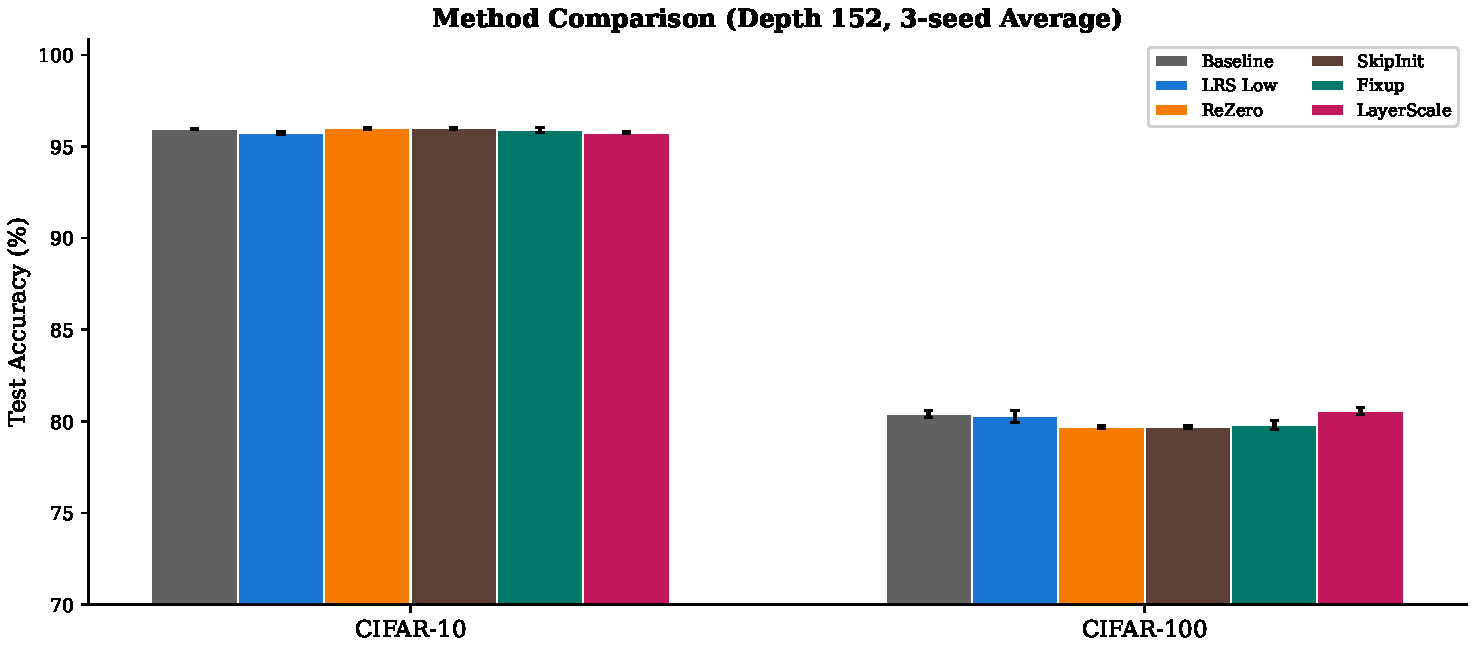
\includegraphics[width=0.85\linewidth]{figures/fig9_comparison.pdf}
    \caption{Accuracy comparison of residual scaling methods at depth 152 on CIFAR-100. All methods perform similarly, but only LRS provides interpretable per-block ratios between $F(x)$ and $x$.}
    \label{fig:method_comparison}
\end{figure}

\subsection{ImageNet: Verifying the Depth--$\alpha$ Scaling Law at Scale}
\label{sec:imagenet}

The CIFAR experiments establish the depth--$\alpha$ scaling law on small-scale data. To verify this law generalizes to large-scale data, we measure converged $\alpha$ on ImageNet at two depths (ResNet-50 and ResNet-101) with LRS Low, using the standard ImageNet stem (7$\times$7 stride-2 conv + max-pool) and matching training configuration (bs $512$, lr $0.2$, $60$ epochs, $5$-epoch warmup). Our primary observable is the converged mean $\alpha$, which our thesis predicts should match the CIFAR pattern at the corresponding depth.

\begin{table}[t]
\centering
\caption{ImageNet $\alpha$ convergence verification. The mean converged $\alpha$ at each ImageNet depth closely matches its CIFAR counterpart at the same nominal depth, confirming that the depth--$\alpha$ scaling law is dataset-independent. Per-block $\alpha$ ranges span the same spread as CIFAR.}
\label{tab:imagenet_alpha}
\begin{tabular}{lcccc}
\toprule
\textbf{Depth} & \textbf{Blocks} & \textbf{ImageNet} $\bar{\alpha}$ & \textbf{CIFAR-100} $\bar{\alpha}$ & \textbf{Match?} \\
\midrule
50  & 16 & 0.303 & 0.342 & \checkmark \\
101 & 33 & $\sim$0.15 & 0.183 & \checkmark \\
\bottomrule
\end{tabular}
\end{table}

At both depths, the converged $\alpha$ on ImageNet closely matches the value observed on CIFAR-100 at the same depth. ResNet-50 yields $\bar{\alpha} = 0.303$ (vs.\ CIFAR $0.342$), and ResNet-101 yields $\bar{\alpha} \approx 0.15$ (vs.\ CIFAR $0.183$). The fact that doubling depth from $50$ to $101$ roughly halves $\bar{\alpha}$ on \emph{both} datasets is the strongest evidence we can offer that the depth--$\alpha$ scaling law reflects an intrinsic architectural property rather than a dataset-specific artifact. ImageNet has $\sim25\times$ more training samples, $10\times$ more classes, and $7\times$ larger input resolution than CIFAR; the persistence of the $\alpha$ pattern across this gap rules out simple dataset-size explanations.

\textbf{Note on classification accuracy.} Top-1 classification accuracy on ImageNet is reported in Appendix~\ref{sec:imagenet_acc} for reproducibility. We emphasize that accuracy is not the goal of this work: LRS is a measurement tool, and we expect---and observe---that adding a measurement instrument can slightly perturb classification accuracy. The relevant finding is the $\alpha$ measurement itself, which confirms our thesis at scale.

\begin{figure}[t]
    \centering
    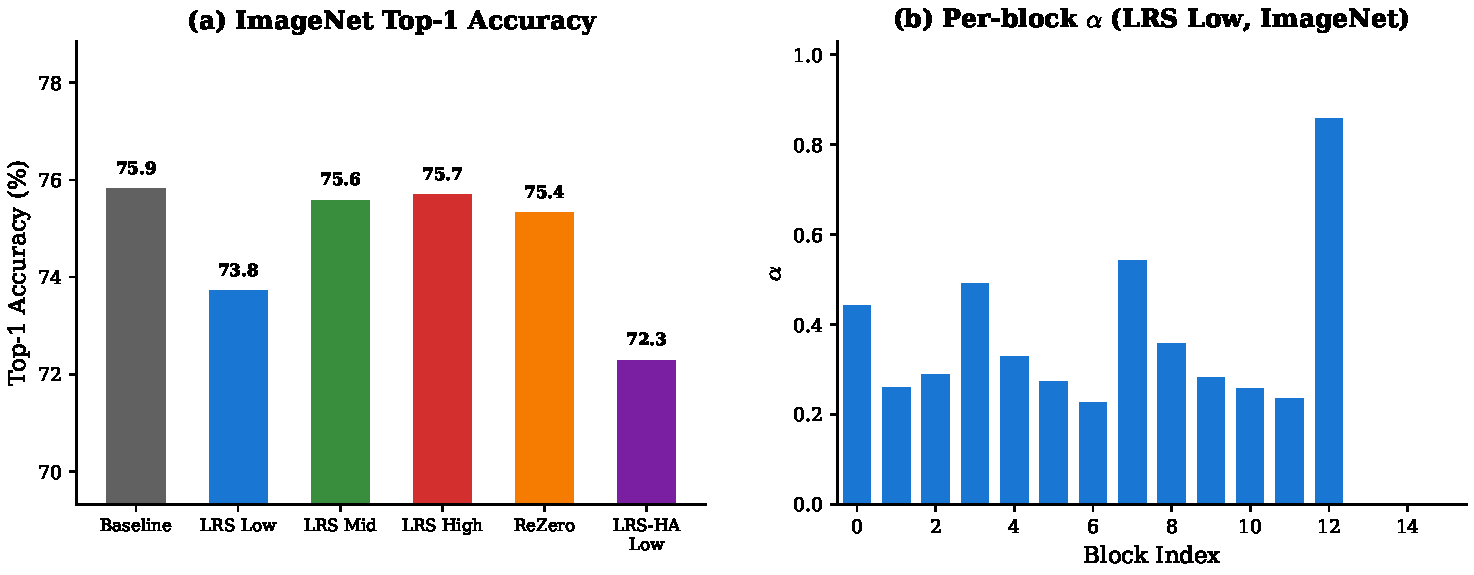
\includegraphics[width=0.85\linewidth]{figures/fig10_imagenet.pdf}
    \caption{ImageNet $\alpha$ convergence at two depths. The mean converged $\alpha$ at each depth closely tracks the corresponding CIFAR-100 value, confirming the depth--$\alpha$ scaling law is dataset-independent.}
    \label{fig:imagenet}
\end{figure}

%% ============================================================
\section{Discussion}
\label{sec:discussion}

\subsection{ResNets Self-Select Their Depth}

The central finding of this work is that deep ResNets do not use their full depth. A 200-layer network (66 blocks) trained with LRS concentrates its transformations in 5--6 blocks---primarily at stage boundaries---and reduces the remaining 60 blocks to near-identity operations. The network has autonomously chosen an effective depth of roughly 8\% of its nominal depth.

The conventional view is that skip connections ``solve'' the degradation problem by enabling gradient flow through deep networks. Our gradient analysis (Figure~\ref{fig:gradient_flow}) confirms that skip connections do stabilize gradient flow: a plain network without skip connections exhibits gradient explosion exceeding $10^{13}$ in early blocks, while ResNet maintains gradients within a manageable range across all 66 blocks. However, LRS reveals that the network uses this stability not to leverage deep computation, but to \emph{bypass} most of its blocks. The near-zero gradients in later blocks of LRS Low (gradient norm $0.6$ at Block~65) reflect $\alpha \approx 0$---the network has chosen not to train these blocks at all.

Furthermore, our identity initialization experiments (Section~\ref{sec:identity_init}) demonstrate that this behavior is not an artifact of poor initialization. Even when the residual branch is initialized as an identity transformation---providing a theoretically better starting point for learning---the network converges to the same effective depth (5--6 active blocks out of 66, mean $\alpha \approx 0.11$--$0.12$). This invariance across initialization schemes strongly suggests that the low effective depth reflects the network's genuine architectural preference.

These observations lead to a reinterpretation of the degradation problem: degradation is not a ``problem to be solved'' but a natural consequence of the network selecting its optimal depth. Skip connections provide the \emph{mechanism} for this self-selection by enabling blocks to act as near-identity operations without disrupting gradient flow. The network does not degrade because it fails to use its depth; rather, it succeeds precisely \emph{because} it can choose not to use unnecessary depth.

This finding resonates with the ``unrolled iterative estimation'' view of residual networks~\cite{greff2017highway} and the path ensemble interpretation~\cite{veit2016residual}. Our contribution is to make this self-selection \emph{directly observable} through the learned $\alpha$ values, rather than inferring it indirectly from path analysis or ablation studies.

\subsection{The Role of Downsampling Blocks}
\label{sec:downsampling_role}

The per-block analysis reveals that not all blocks are equal. Downsampling blocks (at stage boundaries) maintain high $\alpha$ values (0.42--0.96), indicating that spatial and channel dimension changes are essential transformations that cannot be bypassed. In contrast, the many within-stage blocks contribute minimally---most converge to $\alpha < 0.15$, and $\alpha$ decreases progressively further from the downsampling point. The network treats each stage as ``one essential transformation (downsampling) followed by progressively negligible refinements.''

This empirically grounds a design principle that has been implicit in many efficient architectures: \textbf{the number of stages (and thus downsampling operations) matters more than the total number of blocks per stage}. Three lines of prior work converge with this observation. (i) MobileNet~\cite{howard2017mobilenets} and EfficientNet~\cite{tan2019efficientnet} achieve strong accuracy with shallow per-stage block counts, distributing capacity across stages rather than within them. (ii) Stochastic Depth~\cite{huang2016deep} found that randomly dropping later within-stage blocks during training hurts performance far less than dropping stage-transition blocks. (iii) Neural architecture search literature~\cite{tan2019efficientnet} consistently allocates more channels at stage transitions than additional within-stage layers. LRS provides a per-block measurement that explains \emph{why} these design choices succeed: the within-stage blocks they remove are precisely the blocks our $\alpha$ values flag as near-identity.

A practical corollary: when designing or scaling a residual network, increasing nominal depth $L$ within a fixed stage count yields rapidly diminishing returns. Our $D_\text{eff}$ measurements (Table~\ref{tab:deff}) make this explicit---quadrupling blocks from $L{=}50$ to $L{=}200$ increases effective depth from 5.4 to only 7.5. The network's capacity is fundamentally bounded by stage transitions, not by within-stage block count.

\subsection{Why Does Standard ResNet Still Work Well?}

A natural question is: if the optimal $\alpha$ is much less than 0.5, why does the standard ResNet (implicit $\alpha = 0.5$ in the LRS view) perform so well? The answer lies in an important distinction. Standard ResNet uses $y = F(x) + x$, which does not constrain the relative scale of $F(x)$ and $x$. Through batch normalization and weight magnitude adjustment, the network can effectively achieve a small $\|F(x)\|/\|x\|$ ratio without an explicit $\alpha$ parameter. LRS makes this implicit ratio explicit and observable.

Indeed, He et al.~\cite{he2016identity} and De and Smith~\cite{de2020batch} have shown that batch normalization biases residual blocks toward small $F(x)$, effectively implementing a form of identity preference without learnable scaling. LRS confirms and quantifies this phenomenon.

\subsection{Practical Implications}
\label{sec:practical_implications}

Our findings translate into three actionable guidelines, each backed by experimental evidence.

\textbf{(1) $\alpha$-guided structural pruning.} The strongest practical use of LRS is as an \emph{automatic block-importance criterion for pruning}. Unlike magnitude-based pruning or sensitivity analysis, $\alpha$ values are produced as a free byproduct of training---no additional importance scoring is needed. Section~\ref{sec:pruning} validates this concretely: at $\alpha < 0.03$, two blocks (12 conv/BN layers) can be removed from a 200-layer network with \emph{zero} accuracy loss; at $\alpha < 0.05$, 15\% of blocks can be removed with $-1.01\%$ accuracy after a brief fine-tuning. This is a one-shot pruning workflow: train once with LRS, threshold $\alpha$, fine-tune for $\sim$10 epochs. The procedure requires no separate importance estimator, no iterative pruning, and no architecture-specific heuristics.

\textbf{(2) Identity-favoring initialization is essential for deep training.} The catastrophic failure of LRS High at depth 200 (CIFAR-100: 37.50$\pm$29.20\%, Section~\ref{sec:init_sensitivity}) demonstrates that residual-favoring initialization is not merely suboptimal but actively destabilizes training. The mechanism is gradient-preservation: through $L$ blocks, the identity component of the gradient factor compounds as $(1{-}\alpha_0)^L$, vanishing for high $\alpha_0$. For any future work involving learnable residual scaling, initializing $\alpha_0 \leq 0.12$ (equivalently $\theta_0 \leq -2$) is safe across all depths we tested. This guideline aligns with ReZero ($\alpha_0 = 0$) and SkipInit, but is more permissive: $\alpha_0 \approx 0.12$ allows the network to refine from a non-degenerate starting point.

\textbf{(3) Architecture search and design.} The heterogeneous $\alpha$ distribution (high at stage transitions, low within stages) provides a falsifiable design heuristic: \emph{capacity should be allocated at stage boundaries rather than within stages}. Neural architecture search procedures could use $\alpha$-statistics as a regularizer to penalize architectures that allocate too many within-stage blocks. More immediately, the $D_\text{eff}$ metric (Table~\ref{tab:deff}) provides a quick diagnostic: if $D_\text{eff} \ll L$ after training, the network is overparameterized in depth.

\subsection{Limitations}

This study has several limitations, which we address directly.

\textbf{Scale of ImageNet evaluation.} Our ImageNet experiments cover ResNet-50 and ResNet-101 (16 and 33 blocks). The scaling law verifies at both depths, but we have not extended to ResNet-152 or ResNet-200 on ImageNet due to compute cost. Given that the $\bar{\alpha}$ values at the two ImageNet depths track the CIFAR-100 pattern closely (Table~\ref{tab:imagenet_alpha}), we expect the law to continue at deeper ImageNet models, but this remains to be verified directly.

\textbf{Measurement-induced bias.} LRS adds one parameter per block and modifies the optimization landscape, raising the concern that the learned $\alpha$ values reflect this modification rather than the standard ResNet's implicit preferences. Two pieces of evidence argue against this. First, the identity-initialization experiments (Section~\ref{sec:identity_init}) show that mean $\alpha$ converges to nearly identical values (0.114 vs.\ 0.118) regardless of whether the residual branch is initialized randomly (He) or as identity, indicating the convergence target is intrinsic to the architecture rather than to the optimization path. Second, prior work~\cite{de2020batch} independently established that batch normalization biases standard ResNet residuals toward identity---a phenomenon LRS makes explicit but does not create. We interpret LRS as a measurement instrument that makes a preexisting preference observable, not a force that imposes one.

\textbf{Architecture scope.} Our analysis is restricted to bottleneck ResNets. Basic blocks (ResNet-18/34), Vision Transformers, and other residual architectures are not covered. The closely related LayerScale~\cite{touvron2021going} serves a similar stabilization role in ViTs, but its per-channel parameterization does not yield the per-block scalar interpretation LRS provides. Extending LRS to these architectures is straightforward in principle but is left to future work.

\textbf{Threshold dependency.} The ``active block'' threshold $\alpha > 0.3$ in Section~\ref{sec:effective_depth} is admittedly arbitrary. We address this by reporting (i) results across four thresholds (Table~\ref{tab:threshold_sensitivity}) showing the qualitative pattern is invariant, and (ii) a threshold-free metric $D_\text{eff} = \sum_i \alpha_i$ (Table~\ref{tab:deff}) that recovers the same conclusion without any cutoff.

%% ============================================================
\section{Conclusion}
\label{sec:conclusion}

We proposed and empirically supported a concrete answer to why deep ResNets train successfully: \textbf{they autonomously select an effective depth far smaller than their nominal depth, and skip connections provide the architectural freedom that makes this self-selection possible.} Plain networks fail because they have no such freedom---their gradients explode and they cannot choose to bypass redundant layers. ResNets do not avoid the degradation problem by making all layers useful; they avoid it by giving the network the option to refuse depth it does not need.

The thesis rests on three lines of measurable evidence:

\begin{enumerate}
    \item \textbf{Self-selection happens, and it is large.} Across $120$ CIFAR runs (3 seeds, 4 depths, 2 datasets) and ImageNet experiments at depths 50 and 101, deep ResNets compress their effective depth to roughly 8\% of nominal depth. In a 200-layer network, only 5--6 of 66 blocks remain active. The depth--$\alpha$ scaling law ($\bar{\alpha}$ decreases monotonically with depth) is consistent across datasets and scales.
    \item \textbf{Skip connections are the enabling mechanism.} Without skip connections, gradients explode and training is impossible---the network has no opportunity to self-select. With skip connections, the same depth becomes trainable specifically because the network can choose to route information through the identity. Our gradient analysis shows that LRS-trained networks use this stability to make late blocks inert, not to engage them.
    \item \textbf{The selection is intrinsic, not an optimization artifact.} Random and identity initialization of the residual branch converge to nearly identical $\bar{\alpha}$ (0.114 vs.\ 0.118). $\alpha$-guided pruning validates that low-$\alpha$ blocks are genuinely unused: removing $\alpha < 0.03$ blocks incurs zero accuracy loss. Residual-favoring initialization, which obstructs self-selection, causes catastrophic failure at extreme depth.
\end{enumerate}

\textbf{Reframing the degradation problem.} The conventional view casts deep networks as ``working'' only when each added layer contributes positively. Our results suggest a different reading: deep networks work when they are allowed not to use most layers. Capacity that is not used is not capacity that is wasted---it is reserve, and skip connections are the architectural mechanism that makes reserve a viable design choice. This view aligns with the path-ensemble interpretation of Veit et al.~\cite{veit2016residual} but provides a direct, per-block measurement rather than an inferred one.

\textbf{Practical consequences.} Three implications follow directly. (i) For architecture design, adding within-stage depth yields rapidly diminishing returns; capacity should be concentrated at stage transitions, where $\alpha$ remains high. (ii) For model compression, $\alpha$ produced as a byproduct of training is a one-shot pruning criterion that requires no separate importance estimator. (iii) For training stability, identity-favoring initialization is necessary at extreme depth---residual-favoring initialization obstructs the self-selection mechanism.

\textbf{Future work.} Extending LRS to basic-block ResNets (18/34) and Vision Transformers would test whether self-selection is a property of residual architectures broadly or specific to bottleneck ResNets. A theoretical account of \emph{why} the network prefers small $\alpha$ at depth---beyond the gradient-product argument we offer in Section~\ref{sec:method}---remains an open question. We hope LRS, as a measurement instrument, will be useful in pursuing both.

%% ============================================================
\section*{CRediT Authorship Contribution Statement}
\textbf{Jinho Ju}: Conceptualization, Methodology, Software, Validation, Formal analysis, Investigation, Writing -- Original Draft, Visualization.

\section*{Declaration of Competing Interest}
The author declares no competing interests.

\section*{Data and Code Availability}
All code, trained models, and experimental results are publicly available at \url{https://github.com/Wlsghdh/Learnable_Residual_Scaling}.

%% ============================================================
\bibliographystyle{cas-model2-names}

\begin{thebibliography}{12}
\expandafter\ifx\csname natexlab\endcsname\relax\def\natexlab#1{#1}\fi
\providecommand{\url}[1]{\texttt{#1}}
\providecommand{\href}[2]{#2}
\providecommand{\path}[1]{#1}
\providecommand{\DOIprefix}{doi:}
\providecommand{\bibinfo}[2]{#2}

\bibitem[{He et~al.(2016a)}]{he2016deep}
\bibinfo{author}{K.~He}, \bibinfo{author}{X.~Zhang}, \bibinfo{author}{S.~Ren}, \bibinfo{author}{J.~Sun},
\bibinfo{year}{2016}a.
\bibinfo{title}{Deep residual learning for image recognition}.
\newblock In: \bibinfo{booktitle}{Proceedings of the IEEE Conference on Computer Vision and Pattern Recognition (CVPR)}, pp.~\bibinfo{pages}{770--778}.

\bibitem[{He et~al.(2016b)}]{he2016identity}
\bibinfo{author}{K.~He}, \bibinfo{author}{X.~Zhang}, \bibinfo{author}{S.~Ren}, \bibinfo{author}{J.~Sun},
\bibinfo{year}{2016}b.
\bibinfo{title}{Identity mappings in deep residual networks}.
\newblock In: \bibinfo{booktitle}{European Conference on Computer Vision (ECCV)}, pp.~\bibinfo{pages}{630--645}.

\bibitem[{Bachlechner et~al.(2021)}]{bachlechner2021rezero}
\bibinfo{author}{T.~Bachlechner}, \bibinfo{author}{B.P.~Majumder}, \bibinfo{author}{H.H.~Mao}, \bibinfo{author}{G.W.~Cottrell}, \bibinfo{author}{J.~McAuley},
\bibinfo{year}{2021}.
\bibinfo{title}{ReZero is all you need: Fast convergence at large depth}.
\newblock In: \bibinfo{booktitle}{Uncertainty in Artificial Intelligence (UAI)}, pp.~\bibinfo{pages}{1352--1361}.

\bibitem[{De and Smith(2020)}]{de2020batch}
\bibinfo{author}{S.~De}, \bibinfo{author}{S.L.~Smith},
\bibinfo{year}{2020}.
\bibinfo{title}{Batch normalization biases residual blocks towards the identity function in deep networks}.
\newblock In: \bibinfo{booktitle}{Advances in Neural Information Processing Systems (NeurIPS)}, vol.~\bibinfo{volume}{33}.

\bibitem[{Touvron et~al.(2021)}]{touvron2021going}
\bibinfo{author}{H.~Touvron}, \bibinfo{author}{M.~Cord}, \bibinfo{author}{A.~Sablayrolles}, \bibinfo{author}{G.~Synnaeve}, \bibinfo{author}{H.~J\'{e}gou},
\bibinfo{year}{2021}.
\bibinfo{title}{Going deeper with image transformers}.
\newblock In: \bibinfo{booktitle}{Proceedings of the IEEE/CVF International Conference on Computer Vision (ICCV)}, pp.~\bibinfo{pages}{32--42}.

\bibitem[{Zhang et~al.(2019)}]{zhang2019fixup}
\bibinfo{author}{H.~Zhang}, \bibinfo{author}{Y.N.~Dauphin}, \bibinfo{author}{T.~Ma},
\bibinfo{year}{2019}.
\bibinfo{title}{Fixup initialization: Residual learning without normalization}.
\newblock In: \bibinfo{booktitle}{International Conference on Learning Representations (ICLR)}.

\bibitem[{Veit et~al.(2016)}]{veit2016residual}
\bibinfo{author}{A.~Veit}, \bibinfo{author}{M.J.~Wilber}, \bibinfo{author}{S.~Belongie},
\bibinfo{year}{2016}.
\bibinfo{title}{Residual networks behave like ensembles of relatively shallow networks}.
\newblock In: \bibinfo{booktitle}{Advances in Neural Information Processing Systems (NeurIPS)}, vol.~\bibinfo{volume}{29}.

\bibitem[{Srivastava et~al.(2015)}]{srivastava2015highway}
\bibinfo{author}{R.K.~Srivastava}, \bibinfo{author}{K.~Greff}, \bibinfo{author}{J.~Schmidhuber},
\bibinfo{year}{2015}.
\bibinfo{title}{Highway networks}.
\newblock \href{http://arxiv.org/abs/1505.00387}{\tt arXiv:1505.00387}.

\bibitem[{Greff et~al.(2017)}]{greff2017highway}
\bibinfo{author}{K.~Greff}, \bibinfo{author}{R.K.~Srivastava}, \bibinfo{author}{J.~Schmidhuber},
\bibinfo{year}{2017}.
\bibinfo{title}{Highway and residual networks learn unrolled iterative estimation}.
\newblock In: \bibinfo{booktitle}{International Conference on Learning Representations (ICLR)}.

\bibitem[{Huang et~al.(2016)}]{huang2016deep}
\bibinfo{author}{G.~Huang}, \bibinfo{author}{Y.~Sun}, \bibinfo{author}{Z.~Liu}, \bibinfo{author}{D.~Sedra}, \bibinfo{author}{K.Q.~Weinberger},
\bibinfo{year}{2016}.
\bibinfo{title}{Deep networks with stochastic depth}.
\newblock In: \bibinfo{booktitle}{European Conference on Computer Vision (ECCV)}, pp.~\bibinfo{pages}{646--661}.

\bibitem[{Frankle and Carlin(2019)}]{frankle2019lottery}
\bibinfo{author}{J.~Frankle}, \bibinfo{author}{M.~Carlin},
\bibinfo{year}{2019}.
\bibinfo{title}{The lottery ticket hypothesis: Finding sparse, trainable neural networks}.
\newblock In: \bibinfo{booktitle}{International Conference on Learning Representations (ICLR)}.

\bibitem[{Huang et~al.(2017)}]{huang2017densely}
\bibinfo{author}{G.~Huang}, \bibinfo{author}{Z.~Liu}, \bibinfo{author}{L.~van~der~Maaten}, \bibinfo{author}{K.Q.~Weinberger},
\bibinfo{year}{2017}.
\bibinfo{title}{Densely connected convolutional networks}.
\newblock In: \bibinfo{booktitle}{Proceedings of the IEEE Conference on Computer Vision and Pattern Recognition (CVPR)}, pp.~\bibinfo{pages}{4700--4708}.

\bibitem[{Howard et~al.(2017)}]{howard2017mobilenets}
\bibinfo{author}{A.G.~Howard}, \bibinfo{author}{M.~Zhu}, \bibinfo{author}{B.~Chen}, \bibinfo{author}{D.~Kalenichenko}, \bibinfo{author}{W.~Wang}, \bibinfo{author}{T.~Weyand}, \bibinfo{author}{M.~Andreetto}, \bibinfo{author}{H.~Adam},
\bibinfo{year}{2017}.
\bibinfo{title}{MobileNets: Efficient convolutional neural networks for mobile vision applications}.
\newblock \href{http://arxiv.org/abs/1704.04861}{\tt arXiv:1704.04861}.

\bibitem[{Tan and Le(2019)}]{tan2019efficientnet}
\bibinfo{author}{M.~Tan}, \bibinfo{author}{Q.~Le},
\bibinfo{year}{2019}.
\bibinfo{title}{EfficientNet: Rethinking model scaling for convolutional neural networks}.
\newblock In: \bibinfo{booktitle}{International Conference on Machine Learning (ICML)}, pp.~\bibinfo{pages}{6105--6114}.

\end{thebibliography}

\end{document}
